\documentclass[10pt,letterpaper]{article}

% Packages and styling live in preamble.tex; each section has its own file under
% sections/. Edit those directly — this file is the outline of the document.
% Packages, colours and custom commands for this template.
\PassOptionsToPackage{table}{xcolor}
\usepackage[utf8]{inputenc}
\usepackage[T1]{fontenc}
\usepackage[margin=0.85in,headheight=18pt]{geometry}
\usepackage{charter}
\usepackage[scaled=0.92]{helvet}
\usepackage{amsmath,amssymb}
\usepackage{textcomp}
\usepackage{float}
\usepackage{booktabs}
\usepackage{tabularx}
\usepackage{xcolor}
\usepackage{graphicx}
\graphicspath{ {./images/} {./images/waveforms} }

\usepackage{tikz}
\usetikzlibrary{positioning,calc,shapes.geometric,backgrounds}
\usepackage{fancyhdr}
\usepackage{tcolorbox}
\usepackage{enumitem}
\usepackage{titlesec}
\usepackage{lastpage}
\usepackage{hyperref}
\usepackage{xspace}
\usepackage{fontawesome5}

% Define Custom Color Palette
\definecolor{NavyBlue}{HTML}{0F172A}
\definecolor{SteelBlue}{HTML}{1E40AF}
\definecolor{OrangeAccent}{HTML}{D97706}
\definecolor{WarmBg}{HTML}{F8FAFC}
\definecolor{BorderColor}{HTML}{E2E8F0}
\definecolor{LightGray}{HTML}{F1F5F9}
\definecolor{brandprimary}{HTML}{0B2545}
\definecolor{brandsecondary}{HTML}{134074}
\definecolor{brandaccent}{HTML}{8DA9C4}
\definecolor{brandhighlight}{HTML}{EE6C4D}
\definecolor{brandbg}{HTML}{F4F6F9}
\definecolor{brandborder}{HTML}{D3D9E2}
\definecolor{brandmuted}{HTML}{5C6B73}

% Setup Hyperref
\hypersetup{
	colorlinks=true,
	linkcolor=SteelBlue,
	filecolor=SteelBlue,      
	urlcolor=SteelBlue,
	citecolor=SteelBlue,
}

% Style Section Headers
\titleformat{\section}
{\normalfont\large\bfseries\sffamily\color{NavyBlue}}{\thesection}{1em}{}
\titleformat{\subsection}
{\normalfont\normalsize\bfseries\sffamily\color{SteelBlue}}{\thesubsection}{1em}{}
\titleformat{\subsubsection}
{\normalfont\normalsize\itshape\sffamily\color{NavyBlue}}{\thesubsubsection}{1em}{}

% Setup Headers & Footers
\pagestyle{fancy}
\fancyhf{}
\renewcommand{\headrulewidth}{0.5pt}
\renewcommand{\footrulewidth}{0.5pt}
\fancyhead[L]{\sffamily\footnotesize\color{NavyBlue}Doc ID: AXI4LITE-CACHE}
\fancyhead[R]{\sffamily\footnotesize\color{NavyBlue}Rev 1.0}
\fancyfoot[R]{\sffamily\footnotesize\color{NavyBlue}Page \thepage\ of \pageref{LastPage}}

% Define Custom Info Box
\newtcolorbox{infobox}[1]{
	colback=WarmBg,
	colframe=SteelBlue,
	fonttitle=\bfseries\sffamily\color{white},
	colbacktitle=SteelBlue,
	title={#1},
	arc=3pt,
	boxrule=1pt,
	left=10pt,
	right=10pt,
	top=8pt,
	bottom=8pt
}

% Define Custom Warning Box
\newtcolorbox{warningbox}[1]{
	colback=brandhighlight!5,
	colframe=brandhighlight,
	arc=4pt,
	outer arc=4pt,
	title={\sffamily\bfseries\color{white}\faExclamationTriangle\enspace #1},
	coltitle=white,
	fontupper=\sffamily\small,
	boxrule=1.5pt,
	left=12pt,
	right=12pt,
	top=8pt,
	bottom=8pt,
	before skip=10pt,
	after skip=10pt
}

\newcommand{\circled}[2]{%
	\hyperref[#2]{%
		\tikz[baseline=(char.base)]{%
			\node[shape=circle, draw, inner sep=0.2pt] (char) {#1};
		}%
	}%
}

% Define hyper-refs
\newcommand{\TagMemory}{\hyperref[subsec:tag_memory]{Tag Memory}\xspace}
\newcommand{\DataMemory}{\hyperref[subsec:data_memory]{Data Memory}\xspace}
\newcommand{\Comparator}{\hyperref[subsec:comparator]{Comparator}\xspace}
\newcommand{\EvictingBlock}{\hyperref[subsec:evicting_block]{Evicting Block}\xspace}
\newcommand{\PRG}{\hyperref[subsec:prg]{Pseudo-Random Generator}\xspace}
\newcommand{\Arbiter}{\hyperref[subsec:arbiter]{Arbiter}\xspace}
\newcommand{\Buffer}{\hyperref[subsec:buffer]{Buffer}\xspace}
\newcommand{\StatisticsBlock}{\hyperref[subsec:statistics_block]{Statistics Block}\xspace}


\begin{document}
	
	% --- COVER PAGE ---
	\thispagestyle{empty}
	
	\begin{tikzpicture}[remember picture, overlay]
		% Top decorative banner
	\end{tikzpicture}
	
	\vspace{3.5cm}
	
	\begin{flushleft}
		{\Huge\sffamily\bfseries\color{NavyBlue}AXI4-Lite Cache\par}
		\vspace{0.4cm}
		{\Large\sffamily\bfseries\color{OrangeAccent}Microarchitectural Specification\par}
		\vspace{0.4cm}
		\noindent\rule{\textwidth}{1.5pt}
	\end{flushleft}
	
	\vfill
	
	\begin{tcolorbox}[
		colback=WarmBg,
		colframe=BorderColor,
		arc=4pt,
		boxrule=1pt,
		width=\textwidth
		]
		\sffamily
		\begin{tabularx}{\textwidth}{@{}l X l X@{}}
			\textbf{Doc Identifier:} & AXI4LITE-CACHE & \textbf{Release Date:} & October 09, 2026 \\
			\textbf{Version:}        & Rev 1.0 & \textbf{Status:}       & Review \\
			\textbf{Author:} & Danil Zavarnitsyn & \textbf{Reviewer:}    & Maria Stepanova
		\end{tabularx}
	\end{tcolorbox}
	
	\newpage
	
	% --- TABLE OF CONTENTS ---
	\tableofcontents
	\vspace{1cm}
	
	% --- SECTIONS ---
	\section{Introduction}

The AXI4-Lite Cache is a parameterizable set-associative cache designed to reduce the average memory access latency between a processor and an external memory system.

\subsection{Characteristics}
This subsection describes the main features and capabilities supported by the AXI4-Lite Cache.

\begin{table}[htbp]
	\centering
	\label{tab}
	\small
	\begin{tabularx}{\textwidth}{l X}
		\toprule
		\textbf{Characteristic} & \textbf{Description} \\
		\midrule
		
		Configurable Associativity &
		Configurable number of cache ways. \\
		
		Configurable Address and Data Widths &
		Configurable address and data widths. \\
		
		Configurable Number of Sets &
		Configurable number of cache sets. \\
		
		Write-Through Policy with no-allocation&
		Writes are immediately propagated to external memory. \\
		
		NMRU Replacement Policy &
		Approximation of LRU based on the Not Most Recently Used (NMRU) policy. \\
		
		Data-Width Cache Line &
		Cache line size is equal to the data width. \\
		
		AXI4-Lite Interface &
		AXI4-Lite interfaces on the CPU and external memory sides. \\
		
		No Outstanding Transactions &
		Only one cache transaction can be processed at a time.. \\
		
		Hit/Miss Statistics &
		Hit and miss counters are available during simulation only. \\
		
		\bottomrule
	\end{tabularx}
	\caption{Cache characteristics}
\end{table}

% --- SECTION 2 ---

	\newpage
	\section{Functional Description}

This section describes the cache operation for read and write requests, including cache hits, cache misses, and interactions with external memory.

\begin{figure}[h]
	\centering
	\label{fig:cache}
	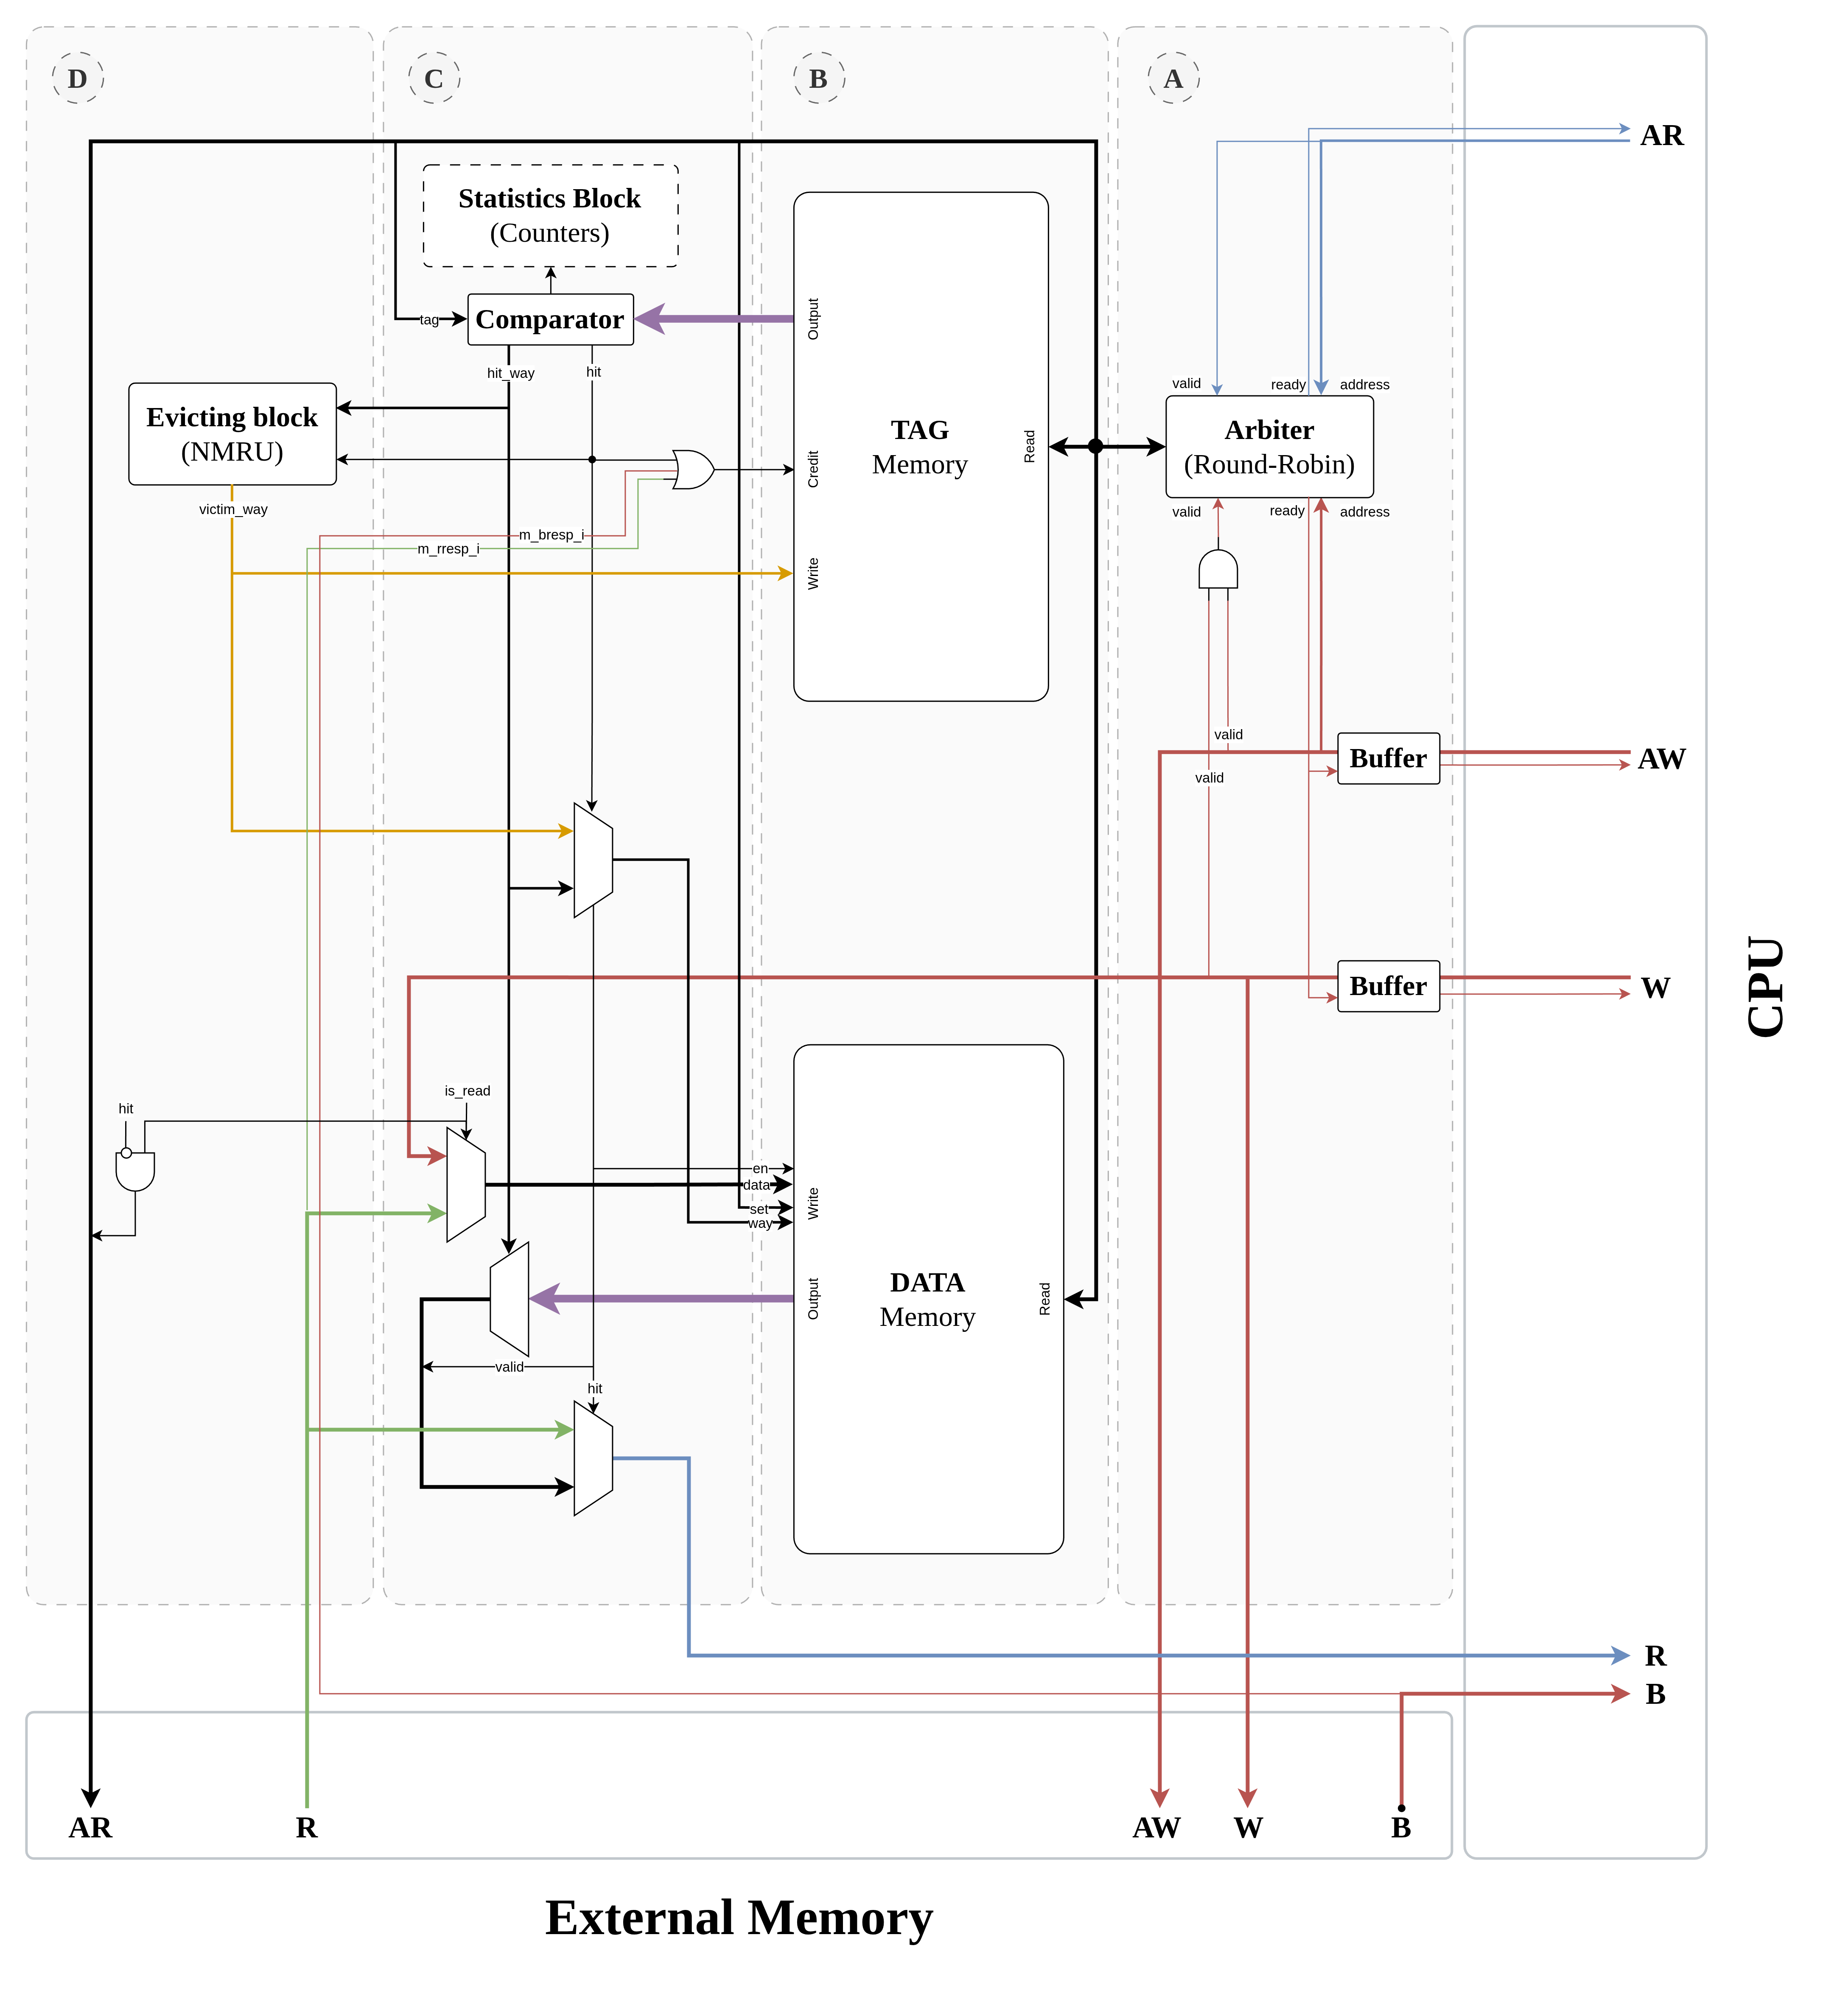
\includegraphics[width=16cm]{Cache.png}
	\caption{Cache scheme}
\end{figure}

\subsection{Request Fetching}

All incoming CPU transactions are initially received by \hyperref[subsec:buffer]{Buffers} located before the \Arbiter. Separate \hyperref[subsec:buffer]{Buffers} are provided for the \verb|AR|, \verb|AW|, and \verb|W| channels (see \circled{A}{fig:cache}).

The \hyperref[subsec:buffer]{Buffers} serve two purposes.
\begin{itemize}
	\item First, they temporarily hold transactions when read and write requests arrive simultaneously, allowing the \Arbiter which operation should be processed first. 
	\item Second, they account for the fact that the \verb|AW| and \verb|W| channels of an AXI4-Lite write transaction may arrive independently and at different times.
\end{itemize}

A write operation is passed to the cache for processing only after both the \verb|AW| and \verb|W| transactions have been received from the CPU.

If only one type of transaction is received, either a read request through the \verb|AR| channel or a complete write request with both \verb|AW| and \verb|W| transactions, it passes through the corresponding buffers and \Arbiter combinatorially.

\subsection{Read Operation}

During a read operation, the CPU provides the requested address through the AXI4-Lite \verb|AR| channel. The address is used simultaneously to initiate a read operation in both the \TagMemory and \DataMemory (see \circled{B}{fig:cache}).

The set index is extracted from the requested address and is used to access the corresponding set in both memories. On the following clock cycle, the \TagMemory provides the tags and valid bits of all ways belonging to the selected set. In parallel, the \DataMemory provides the data stored in all ways of the same set.

The set of ways obtained from the \TagMemory, together with the requested tag extracted from the address, is provided to the \Comparator. The \Comparator compares the requested tag with the tag stored in each way in parallel and determines whether the requested cache line is present (see \circled{C}{fig:cache}). 

\subsubsection{Read Hit}

In case of a cache hit, the \Comparator asserts the hit signal and provides the index of the way containing the requested tag through \verb|hit_way|.

The \verb|hit_way| value is provided to the \EvictingBlock to update the most recently used way for the corresponding set. At the same time, \verb|hit_way| is used to select the required data from the set of ways returned by the \DataMemory. The selected data is then provided to the CPU through the AXI4-Lite \verb|R| channel (see \circled{C}{fig:cache}).

Since the \TagMemory and \DataMemory are accessed in parallel, the cache can determine the requested way and select the corresponding data within a single clock cycle.

\subsubsection{Read Miss}

In case of a cache miss, the \EvictingBlock is activated to select the way that will be replaced in the selected set. The victim way is selected by \PRG while ensuring that the most recently used way is not selected for replacement (see \circled{D}{fig:cache}). The generated victim way is then used to select the cache way that will be overwritten in the \TagMemory.

At the same time, the address of the requested cache line is provided to the external memory through the AXI4-Lite \verb|AR| channel. The data returned by the external memory on the \verb|R| channel is written into the selected way of the \DataMemory and is simultaneously forwarded to the CPU through the CPU-side AXI4-Lite \verb|R| channel (see \circled{C}{fig:cache}).

\subsection{Write Operation}
During a write operation, the data is written directly to the external memory through the AXI4-Lite interface and allocates in the cache according to the write-through policy.

When the CPU provides the write address and data through the AXI4-Lite \verb|AW| and \verb|W| channels, the write address is simultaneously provided to the \TagMemory (see \circled{B}{fig:cache}). The set index extracted from the address is used to access the corresponding set, and the requested tag is compared with the tags of all ways by the \Comparator, following the same procedure as for a read operation (see \circled{C}{fig:cache}).

\subsubsection{Write Hit}

If a matching tag is found, the corresponding way is identified by \verb|hit_way|. The new data is written both to the selected way of the \DataMemory (see \circled{C}{fig:cache}) and to the external memory. The write address and data received from the CPU through the AXI4-Lite \verb|AW| and \verb|W| channels are forwarded to the corresponding channels of the external memory interface.

\subsubsection{Write Miss}

If no matching tag is found, the \EvictingBlock is activated to select the way that will be replaced in the selected set (see \circled{D}{fig:cache}). The victim way is selected by \PRG while ensuring that the most recently used way is not selected for replacement.

The tag of the current write address is written into the selected way of the \TagMemory, and the corresponding data is written into the selected way of the \DataMemory (see \circled{C}{fig:cache}). At the same time, the write address and data received from the CPU through the AXI4-Lite \verb|AW| and \verb|W| channels are forwarded to the corresponding channels of the external memory interface.

\subsection{Hits Counting}
The cache provides hit and miss counting functionality for simulation and performance analysis. This functionality is implemented in the \StatisticsBlock.

The \StatisticsBlock receives hit and miss information from the \Comparator, which determines whether the requested tag is present in the selected cache set.

\begin{infobox}{Simulation Only}
	The \StatisticsBlock is intended exclusively for simulation purposes and is not included in the synthesized cache design. Therefore, it does not introduce any hardware overhead in the final implementation.
\end{infobox}
	\section{Clock and Reset}

The AXI4-Lite Cache operates within a single clock domain and a single reset domain. No clock domain crossings are present. The cache uses the \verb|clk_i| signal as its clock and the \verb|rstn_i| signal as an active-low synchronous reset.

During reset, the entire \TagMemory is cleared, including all stored tags and valid bits. The contents of the \DataMemory do not need to be reset, as they are considered invalid until a corresponding valid entry is created in the \TagMemory.
	\section{Parameters}

The following table lists the parameters used to configure the AXI4-Lite Cache implementation.

\begin{table}[htbp]
	\centering
	\small
	\begin{tabularx}{\textwidth}{l c c X}
		\toprule
		\textbf{Parameter} & \textbf{Valid Range} & \textbf{Default} & \textbf{Description} \\
		\midrule
		
		\verb|ADDR_WIDTH| &
		Positive integer &
		\verb|32| &
		Width of the memory address. \\
		
		\verb|DATA_WIDTH| &
		32, 64 &
		\verb|32| &
		Width of the data bus. \\
		
		\verb|SET_NUM| &
		Power of 2 &
		\verb|4| &
		Number of cache sets. \\
		
		\verb|WAY_NUM| &
		Power of 2 &
		\verb|4| &
		Number of cache ways (associativity). \\
		
		\verb|DEBUG_ON| &
		0, 1 &
		\verb|0| &
		Enables the \StatisticsBlock when set to \verb|1|. \\
		
		\bottomrule
	\end{tabularx}
	\caption{RTL configuration parameters}
	\label{tab:rtl_parameters}
\end{table}

The following auxiliary parameters are introduced for documentation purposes only. They are used to simplify the description of signal widths and cache organization and do not represent parameters of the RTL implementation.

\begin{table}[htbp]
	\centering
	\small
	\begin{tabularx}{\textwidth}{l c X}
		\toprule
		\textbf{Parameter} & \textbf{Definition} & \textbf{Description} \\
		\midrule
		
		\verb|SET_WIDTH| &
		$\log_2(\text{\verb|SET_NUM|})$ &
		Width of the cache set index. \\
		
		\verb|WAY_WIDTH| &
		$\log_2(\text{\verb|WAY_NUM|})$ &
		Width of the way index. \\
		
		\bottomrule
	\end{tabularx}
	\caption{Auxiliary documentation parameters}
	\label{tab:documentation_parameters}
\end{table}

	\newpage
	\section{Ports Description}

The cache acts as an AXI4-Lite slave on the CPU side and as an AXI4-Lite master on the external memory side. The following table describes all ports of the cache and their respective directions, widths, and functions.

\begin{table}[htbp]
	\centering
	\label{tab:cache_ports}
	\small
	\begin{tabularx}{\textwidth}{l c c X}
		\toprule
		\textbf{Ports} & \textbf{Direction} & \textbf{Width} & \textbf{Description} \\
		\midrule
		
		\verb|clk_i| &
		Input &
		\verb|1| &
		System clock used to synchronize the cache operation. \\
		
		\verb|rstn_i| &
		Input &
		\verb|1| &
		Active-low synchronous reset signal. \\
		
		\midrule
		\multicolumn{4}{l}{\textbf{CPU-side AXI4-Lite interface}} \\
		\midrule
		
		\verb|s_axi_awaddr_i| &
		Input &
		\verb|ADDR_WIDTH| &
		Write address provided by the CPU. \\
		
		\verb|s_axi_awvalid_i| &
		Input &
		\verb|1| &
		Indicates that a valid write address is available. \\
		
		\verb|s_axi_awready_o| &
		Output &
		\verb|1| &
		Indicates that the cache is ready to accept a write address. \\
		
		\verb|s_axi_wdata_i| &
		Input &
		\verb|DATA_WIDTH| &
		Write data provided by the CPU. \\
		
		\verb|s_axi_wstrb_i| &
		Input &
		\verb|DATA_WIDTH / 8| &
		Write byte strobes indicating which bytes of the write data are valid. \\
		
		\verb|s_axi_wvalid_i| &
		Input &
		\verb|1| &
		Indicates that valid write data is available. \\
		
		\verb|s_axi_wready_o| &
		Output &
		\verb|1| &
		Indicates that the cache is ready to accept write data. \\
		
		\verb|s_axi_bresp_o| &
		Output &
		\verb|2| &
		Write response indicating the result of the write transaction. \\
		
		\verb|s_axi_bvalid_o| &
		Output &
		\verb|1| &
		Indicates that a valid write response is available. \\
		
		\verb|s_axi_bready_i| &
		Input &
		\verb|1| &
		Indicates that the CPU is ready to accept the write response. \\
		
		\verb|s_axi_araddr_i| &
		Input &
		\verb|ADDR_WIDTH| &
		Read address provided by the CPU. \\
		
		\verb|s_axi_arvalid_i| &
		Input &
		\verb|1| &
		Indicates that a valid read address is available. \\
		
		\verb|s_axi_arready_o| &
		Output &
		\verb|1| &
		Indicates that the cache is ready to accept a read address. \\
		
		\verb|s_axi_rdata_o| &
		Output &
		\verb|DATA_WIDTH| &
		Read data returned to the CPU. \\
		
		\verb|s_axi_rresp_o| &
		Output &
		\verb|2| &
		Read response indicating the result of the read transaction. \\
		
		\verb|s_axi_rvalid_o| &
		Output &
		\verb|1| &
		Indicates that valid read data is available. \\
		
		\verb|s_axi_rready_i| &
		Input &
		\verb|1| &
		Indicates that the CPU is ready to accept the read data. \\
		
		\midrule
		\multicolumn{4}{l}{\textbf{External memory-side AXI4-Lite interface}} \\
		\midrule
		
		\verb|m_axi_awaddr_o| &
		Output &
		\verb|ADDR_WIDTH| &
		Write address provided to the external memory. \\
		
		\verb|m_axi_awvalid_o| &
		Output &
		\verb|1| &
		Indicates that a valid write address is available. \\
		
		\verb|m_axi_awready_i| &
		Input &
		\verb|1| &
		Indicates that the external memory is ready to accept a write address. \\
		
		\verb|m_axi_wdata_o| &
		Output &
		\verb|DATA_WIDTH| &
		Write data provided to the external memory. \\
		
		\verb|m_axi_wstrb_o| &
		Output &
		\verb|DATA_WIDTH / 8| &
		Write byte strobes indicating which bytes of the write data are valid. \\
		
		\verb|m_axi_wvalid_o| &
		Output &
		\verb|1| &
		Indicates that valid write data is available. \\
		
		\verb|m_axi_wready_i| &
		Input &
		\verb|1| &
		Indicates that the external memory is ready to accept write data. \\
		
		\verb|m_axi_bresp_i| &
		Input &
		\verb|2| &
		Write response returned by the external memory. \\
		
		\verb|m_axi_bvalid_i| &
		Input &
		\verb|1| &
		Indicates that a valid write response is available. \\
		
		\verb|m_axi_bready_o| &
		Output &
		\verb|1| &
		Indicates that the cache is ready to accept the write response. \\
		
		\verb|m_axi_araddr_o| &
		Output &
		\verb|ADDR_WIDTH| &
		Read address provided to the external memory. \\
		
		\verb|m_axi_arvalid_o| &
		Output &
		\verb|1| &
		Indicates that a valid read address is available. \\
		
		\verb|m_axi_arready_i| &
		Input &
		\verb|1| &
		Indicates that the external memory is ready to accept a read address. \\
		
		\verb|m_axi_rdata_i| &
		Input &
		\verb|DATA_WIDTH| &
		Read data returned by the external memory. \\
		
		\verb|m_axi_rresp_i| &
		Input &
		\verb|2| &
		Read response returned by the external memory. \\
		
		\verb|m_axi_rvalid_i| &
		Input &
		\verb|1| &
		Indicates that valid read data is available. \\
		
		\verb|m_axi_rready_o| &
		Output &
		\verb|1| &
		Indicates that the cache is ready to accept the read data. \\
		
		\bottomrule
	\end{tabularx}
	\caption{Cache ports}
\end{table}

	\newpage
	\section{Submodules}

This section describes the micro-architecture and functionality of the submodules used in the cache implementation. For each module, its purpose, internal organization, inputs and outputs, and interaction with other components are presented.

%%%%%%%%%%%%%%%%%%%%%%%%%
%% C O M P A R A T O R %%
%%%%%%%%%%%%%%%%%%%%%%%%%

\subsection{Comparator}
\label{subsec:comparator}

The Comparator module is responsible for determining whether the requested tag is present in the selected cache set. The module receives the requested tag and the array of tags corresponding to all ways of the selected set from the Tag Memory.

\begin{figure}[h]
	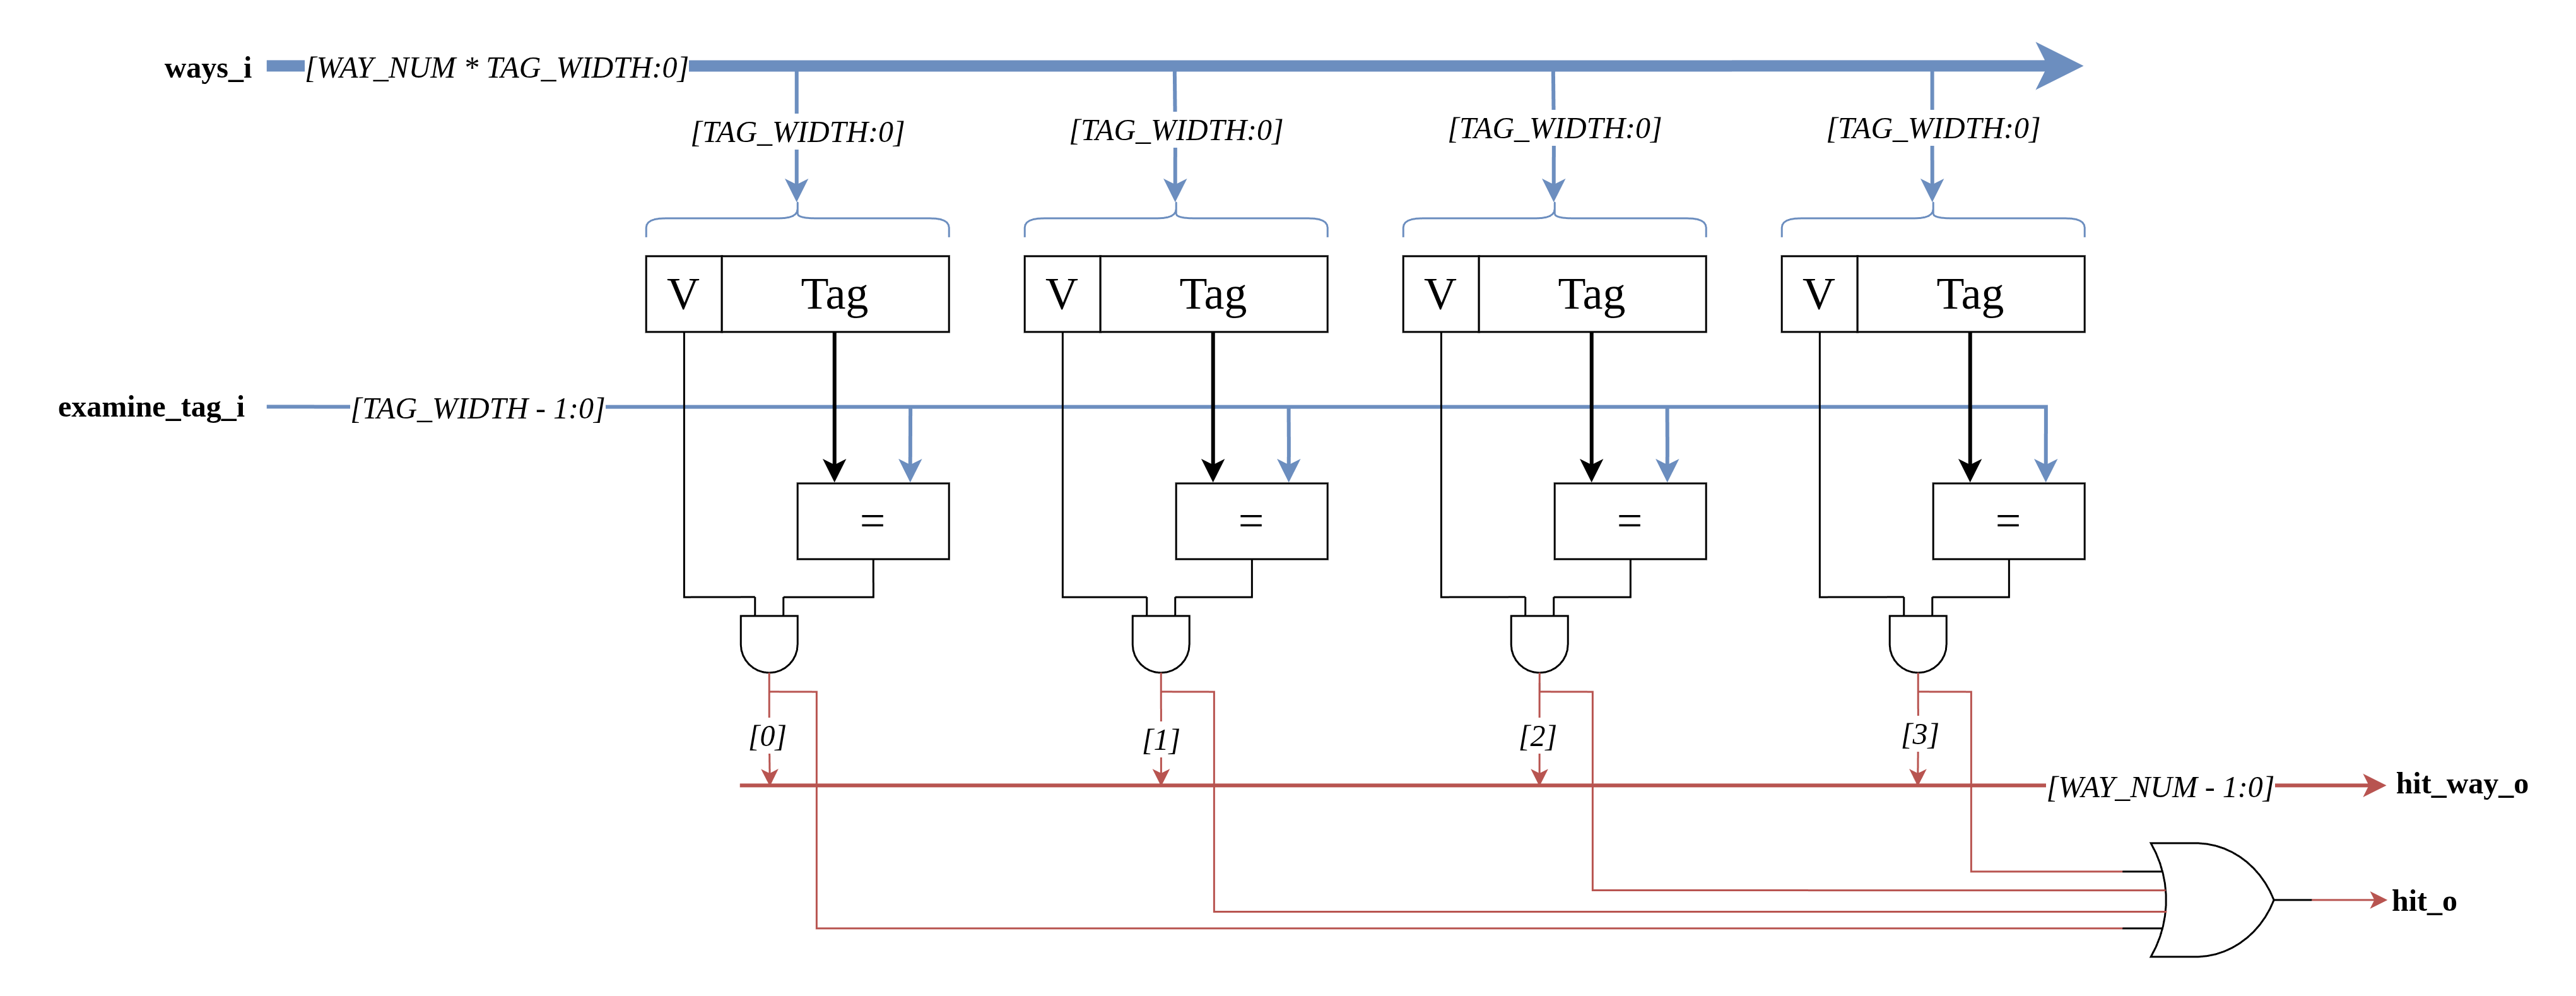
\includegraphics[width=16cm]{Comparator.png}
	\caption{Comparator scheme (4-way cache)}
\end{figure}

The comparison is performed in parallel. For each way, a dedicated comparator compares the tag stored in the corresponding way with the requested tag. The results of the individual comparisons form a match vector. Each bit of this vector corresponds to one way and is asserted when the tag stored in the corresponding way matches the requested tag. Thus, the output of the module represents the location of the matching tag using a one-hot encoding.

\begin{table}[htbp]
	\centering
	\small
	\begin{tabularx}{\textwidth}{l c c X}
		\toprule
		\textbf{Parameter} & \textbf{Valid Range} & \textbf{Default} & \textbf{Description} \\
		\midrule
		
		\verb|TAG_WIDTH| &
		Positive integer &
		--- &
		Width of the cache tag. \\
		
		\verb|WAY_NUM| &
		Positive integer &
		--- &
		Number of cache ways compared in parallel. \\
		
		\bottomrule
	\end{tabularx}
	\caption{Comparator parameters}
	\label{tab:comparator_parameters}
\end{table}

\begin{table}[htbp]
	\centering
	\label{tab:comparator_ports}
	\small
	\begin{tabularx}{\textwidth}{l c c X}
		\toprule
		\textbf{Ports} & \textbf{Direction} & \textbf{Width} & \textbf{Description} \\
		\midrule
		\verb| ways_i | & Input & \verb| WAY_NUM * (TAG_WIDTH + 1) | & Tags and valid bits of all ways belonging to the selected set. \\
		\verb| examine_tag_i| & Input & \verb| TAG_WIDTH | & Tag of the requested cache line to be compared against all ways. \\
		\verb| hit_way_o | & Output & \verb| WAY_NUM | & One-hot encoded indication of the way containing the requested tag.. \\
		\verb| hit_o | & Output & \verb| 1 | & Indicates whether the requested tag was found in any way of the selected set. \\
		\bottomrule
	\end{tabularx}
	\caption{Comparator ports}
\end{table}
%%%%%%%%%%%%%%%%%%%%%%%%%%%%%%%%%%
%% E V I C T I N G    B L O C K %%
%%%%%%%%%%%%%%%%%%%%%%%%%%%%%%%%%%

\subsection{Evicting Block}
\label{subsec:evicting_block}

The Evicting Block is responsible for selecting a victim way when a cache miss occurs and a new cache line has to be allocated. The module implements the \textit{Not Most Recently Used} (NMRU) replacement policy.

\begin{figure}[h]
	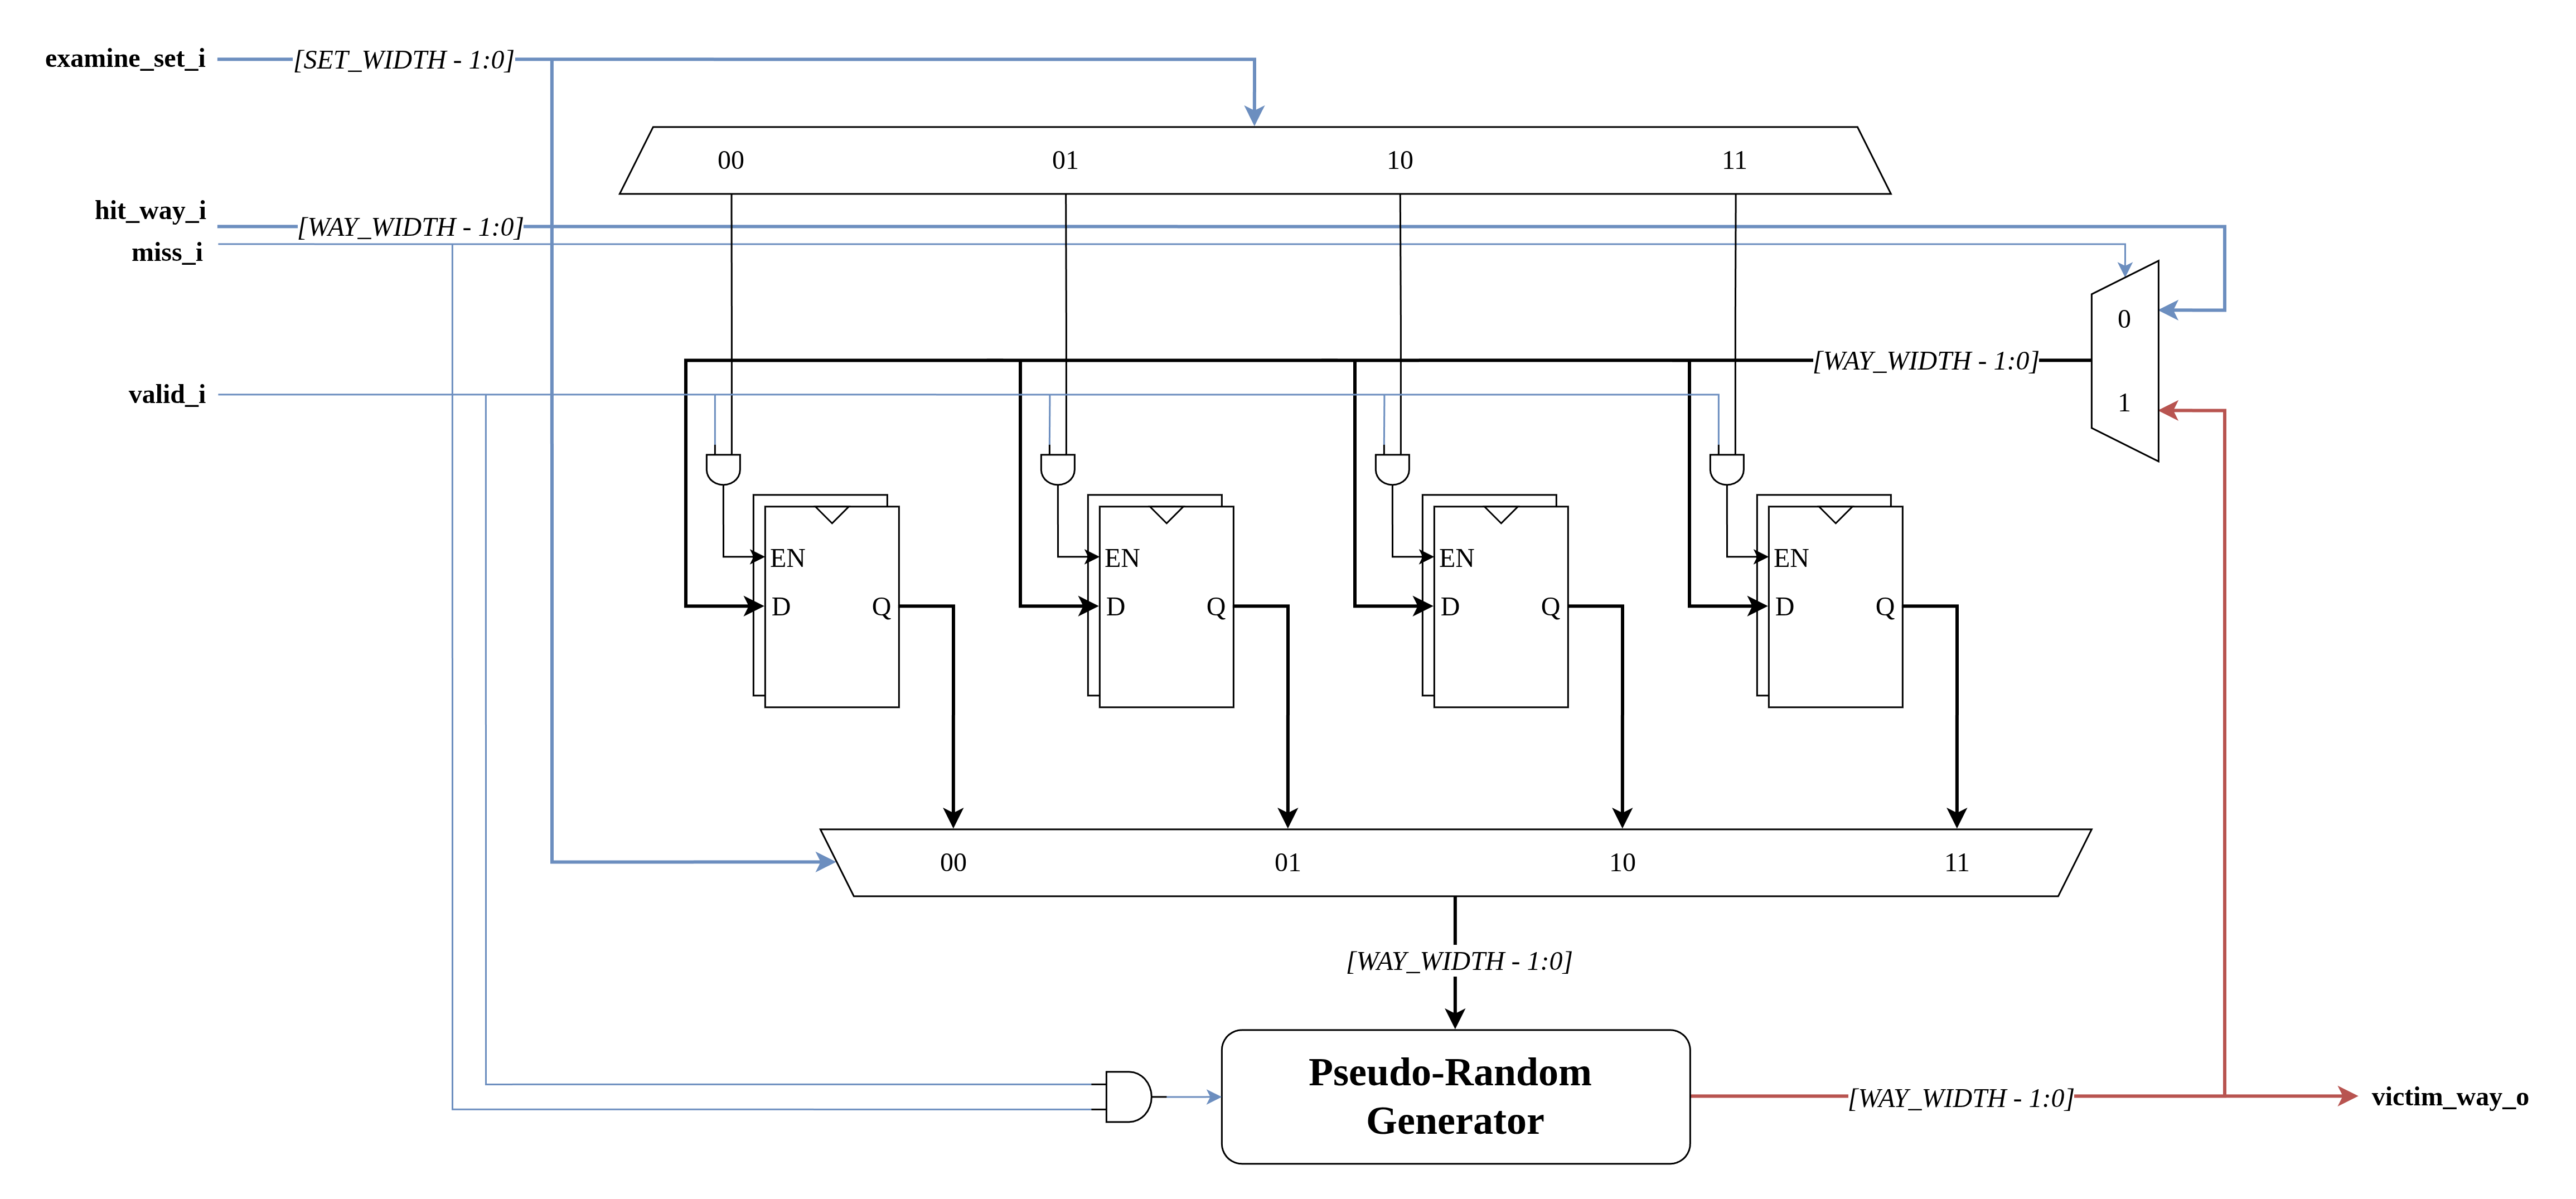
\includegraphics[width=16cm]{NMRU.png}
	\caption{Evicting Block scheme (4-set cache)}
\end{figure}

\begin{table}[htbp]
	\centering
	\small
	\begin{tabularx}{\textwidth}{l c c X}
		\toprule
		\textbf{Parameter} & \textbf{Valid Range} & \textbf{Default} & \textbf{Description} \\
		\midrule
		
		\verb|SET_NUM| &
		Positive integer &
		--- &
		Number of cache sets for which the replacement state is maintained. \\
		
		\verb|WAY_NUM| &
		Positive integer &
		--- &
		Number of cache ways used for victim selection. \\
		
		\bottomrule
	\end{tabularx}
	\caption{Evicting Block parameters}
	\label{tab:evicting_block_parameters}
\end{table}

\begin{table}[htbp]
	\centering
	\label{tab:evicting_block_ports}
	\small
	\begin{tabularx}{\textwidth}{l c c X}
		\toprule
		\textbf{Ports} & \textbf{Direction} & \textbf{Width} & \textbf{Description} \\
		\midrule
		\verb| examine_set_i | & Input & \verb| SET_WIDTH | & Index of the current cache set. \\
		\verb| hit_way_i | & Input & \verb| WAY_WIDTH | & Index of the way containing the requested tag on a cache hit. \\
		\verb| miss_i | & Input & \verb| 1 | & Indicates that the current cache access resulted in a cache miss. \\
		\verb| valid_i | & Input & \verb| 1 | & Indicates whether the selected cache line contains valid data. \\
		\verb| victim_way_o | & Output & \verb| WAY_WIDTH | & Index of the way selected for replacement on a cache miss. \\
		\bottomrule
	\end{tabularx}
	\caption{Evicting Block ports}
\end{table}

The module maintains a separate register for each cache set. Each register stores the index of the way that was most recently used within the corresponding set.

When a cache access results in a hit, the way containing the requested tag becomes the most recently used way.

When a cache miss occurs, the module receives the index of the selected set and reads the corresponding MRU (Most Recently Used) register. The stored way index is then used as a constraint for victim selection: the victim way must not be equal to the most recently used way.

To select the victim, the module contains a \PRG. The generator is activated on a cache miss and produces a candidate way index.

Once a valid victim way has been generated, its index is driven to the module output and is used by the cache control logic to select the way that will be replaced. The selected victim way also becomes the new most recently used way. Therefore, the current MRU register is updated with the generated victim index. This ensures that the most recently accessed or allocated way is excluded from being selected as the victim during the next replacement operation for the same set.
%%%%%%%%%%%%%%%%%%%%%%%%%%%%%%%%%%%%%%%%%%%%%%%%%%%%
%% P S E U D O - R A N D O M    G E N E R A T O R %%
%%%%%%%%%%%%%%%%%%%%%%%%%%%%%%%%%%%%%%%%%%%%%%%%%%%%

\subsection{Pseudo-Random Generator}
\label{subsec:prg}

The Pseudo-Random Generator is responsible for generating a candidate (victim way) used by the \EvictingBlock during cache line replacement. The generator is based on a \textit{Linear Feedback Shift Register} (LFSR), which provides a compact hardware implementation for generating pseudo-random sequences.

\begin{figure}[h]
	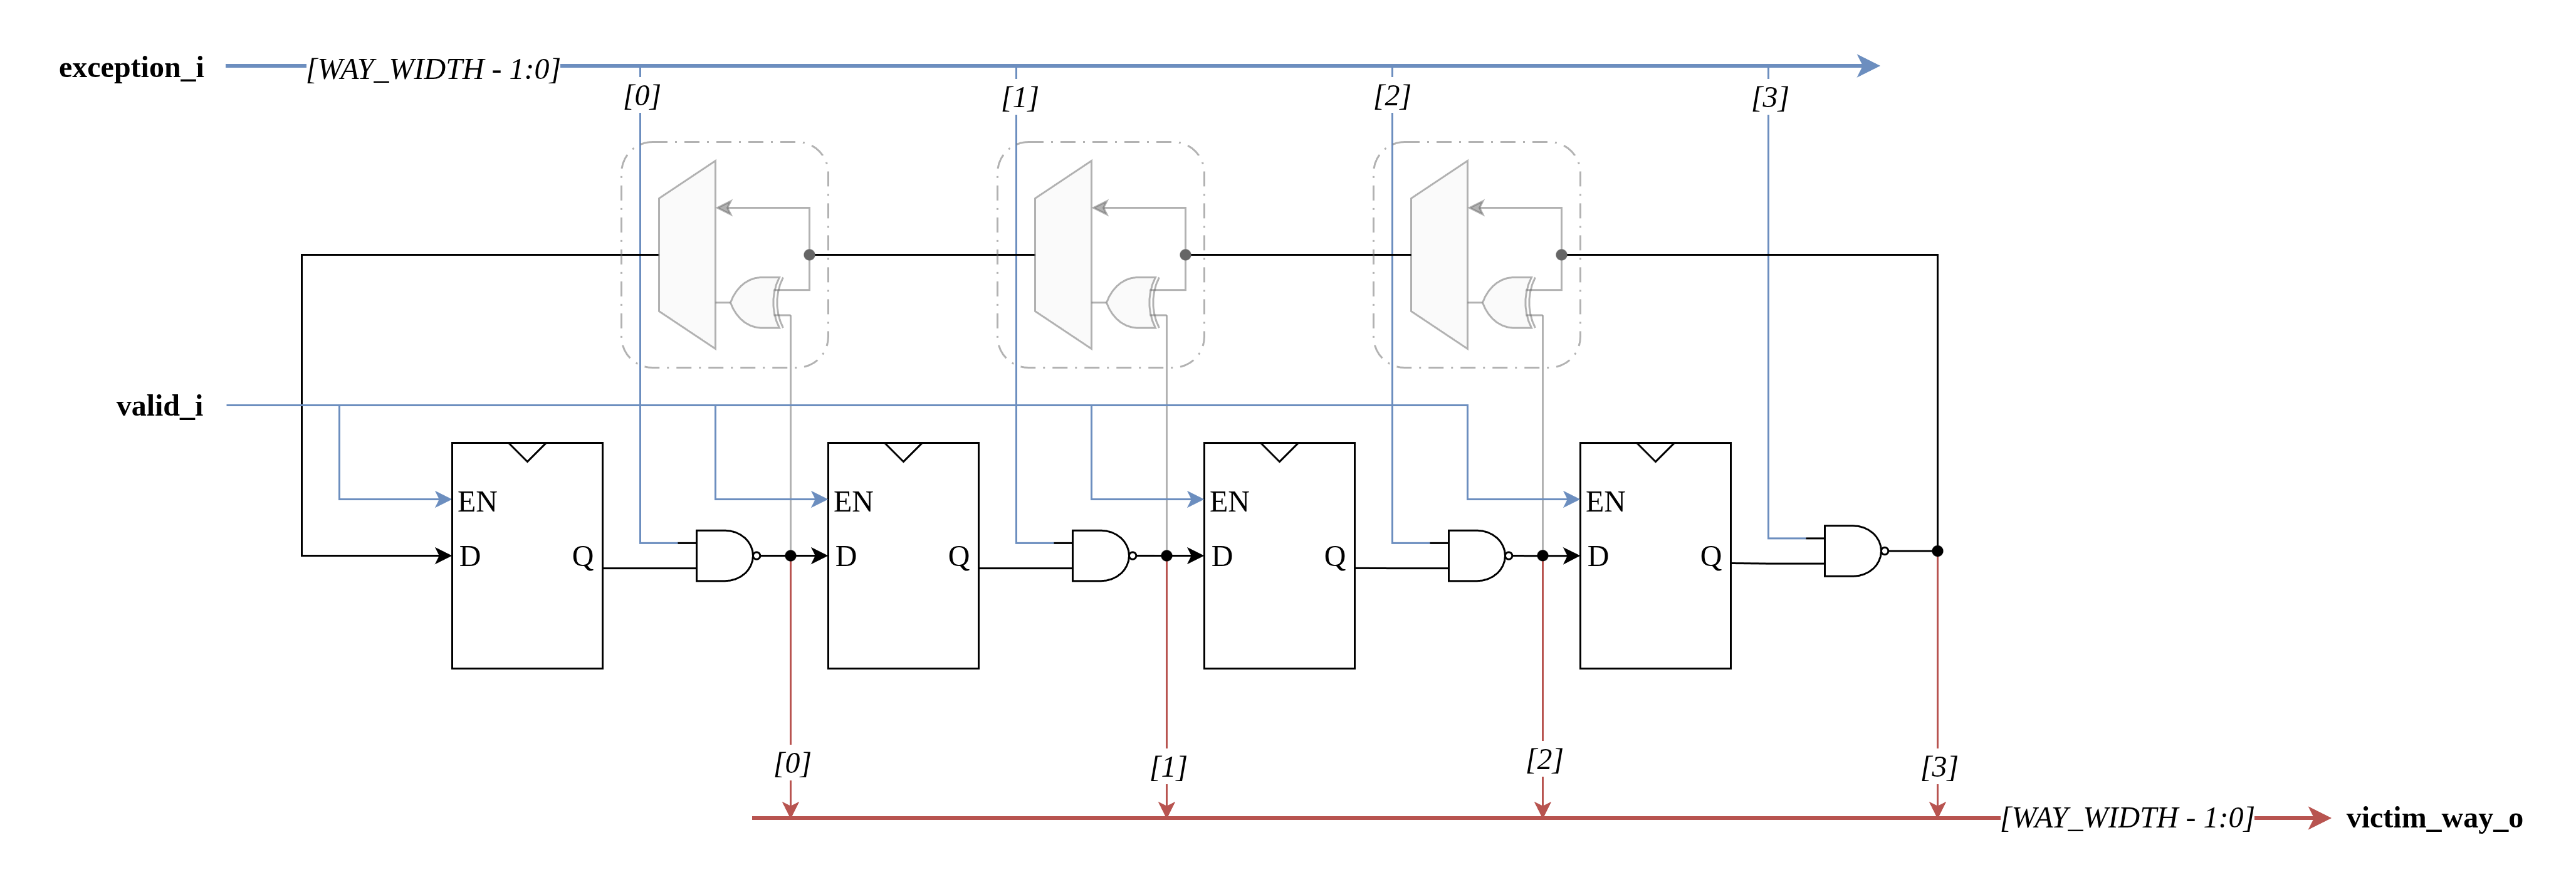
\includegraphics[width=16cm]{PRG.png}
	\caption{Pseudo-Random Generator scheme}
\end{figure}

\begin{table}[htbp]
	\centering
	\small
	\begin{tabularx}{\textwidth}{l c c X}
		\toprule
		\textbf{Parameter} & \textbf{Valid Range} & \textbf{Default} & \textbf{Description} \\
		\midrule
		
		\verb|LFSR_WIDTH| &
		Positive integer &
		\verb|WAY_WIDTH| &
		Number of flip-flops in the LFSR. \\
		
		\verb|LFSR_POLY| &
		Configurable &
		--- &
		Selects the feedback polynomial used by the LFSR. \\
		
		\bottomrule
	\end{tabularx}
	\caption{LFSR configuration parameters}
	\label{tab:lfsr_parameters}
\end{table}
	

\begin{table}[htbp]
	\centering
	\label{tab:prg_ports}
	\small
	\begin{tabularx}{\textwidth}{l c c X}
		\toprule
		\textbf{Ports} & \textbf{Direction} & \textbf{Width} & \textbf{Description} \\
		\midrule
		\verb| exception_i | & Input & \verb| WAY_WIDTH | & Way index that must be excluded from the generated victim way. \\
		\verb| valid_i | & Input & \verb| 1 | & Indicates whether the selected exception way is valid. \\
		\verb| victim_way_o | & Output & \verb| WAY_WIDTH | & Pseudo-randomly generated way index selected as the victim way. \\
		\bottomrule
	\end{tabularx}
	\caption{Pseudo-Random Generator ports}
\end{table}

For a cache with \verb|WAY_NUM| ways, the minimum LFSR width is

\begin{equation}
	N = \log_2( \verb| WAY_NUM |)
\end{equation}

flip-flops. The feedback function of the LFSR is configurable, allowing different feedback polynomials to be selected. The polynomial configuration is implemented using multiplexers placed between adjacent stages of the shift register. For the $i$-th polynomial coefficient, the corresponding multiplexer determines whether the feedback path contains an XOR operation or a direct connection.

The NAND-based transformation provides a simple mechanism for modifying the generated value when it coincides with the prohibited way. If a generated bit matches the corresponding bit of the prohibited way, the NAND logic inverts the affected bit. Therefore, if the complete generated victim way coincides with the prohibited way, the corresponding matching bits are inverted, resulting in a different way index.

The NAND-based feedback also prevents the LFSR from becoming permanently locked in the all-zero state. In a conventional LFSR, the state consisting entirely of zeros is a lock-up state: since all feedback values remain zero, the register cannot transition to another state. In the proposed design, the feedback logic additionally depends on the prohibited way index. Even when the generated way and the prohibited way do not completely match, any matching individual bits can still be inverted by the NAND logic. Consequently, when the LFSR reaches the all-zero state, the interaction with the prohibited way can introduce non-zero bits into the next LFSR state. Therefore, the generator can leave the conventional all-zero lock-up state without requiring separate zero-state recovery logic.

\begin{warningbox}{Victim Way Distribution}
	The NMRU replacement policy relies on the pseudo-random generator providing a sufficiently uniform distribution of victim ways. Ideally, each possible way index should have approximately the same probability of being generated.
	
	This property is not guaranteed by the proposed generator architecture. In the proposed implementation, additional NAND logic is introduced between the LFSR stages to account for the prohibited way. This modification changes the state transition function of the original LFSR and can therefore introduce a bias into the distribution of generated victim ways.
	
	Therefore, before configuring the cache parameters (\verb|SET_NUM|, \verb|WAY_NUM|), the distribution of the generated victim way values must be verified for the selected LFSR configuration. The verification should include a sufficiently long generated sequence and should confirm that all valid way indices occur with approximately equal frequency.
	
	If a significant bias is observed, the distribution can be adjusted by selecting a different feedback polynomial. Another possible solution is to increase the length of the LFSR.
\end{warningbox}
%%%%%%%%%%%%%%%%%%%%%%%%%%%%
%% D A T A    M E M O R Y %%
%%%%%%%%%%%%%%%%%%%%%%%%%%%%

\subsection{Data Memory}
\label{subsec:data_memory}

The Data Memory block encapsulates the multi-bank memory used to store cache data. Each bank stores the data corresponding to a specific way across all cache sets.

Each memory bank is implemented as a pseudo-dual-port memory with a single memory access port that can be used for either a read or a write operation. Read requests are issued by the CPU-side cache logic, while write requests are generated from the R-channel of the external memory-side AXI4-Lite interface. The access type is selected according to the current cache operation.

When a read request is received, the corresponding set index is used to address each memory bank. On the following clock cycle, the Data Memory block provides the data stored in all ways of the selected set.

Both read and write operations have a latency of one clock cycle.

\begin{figure}[H]
	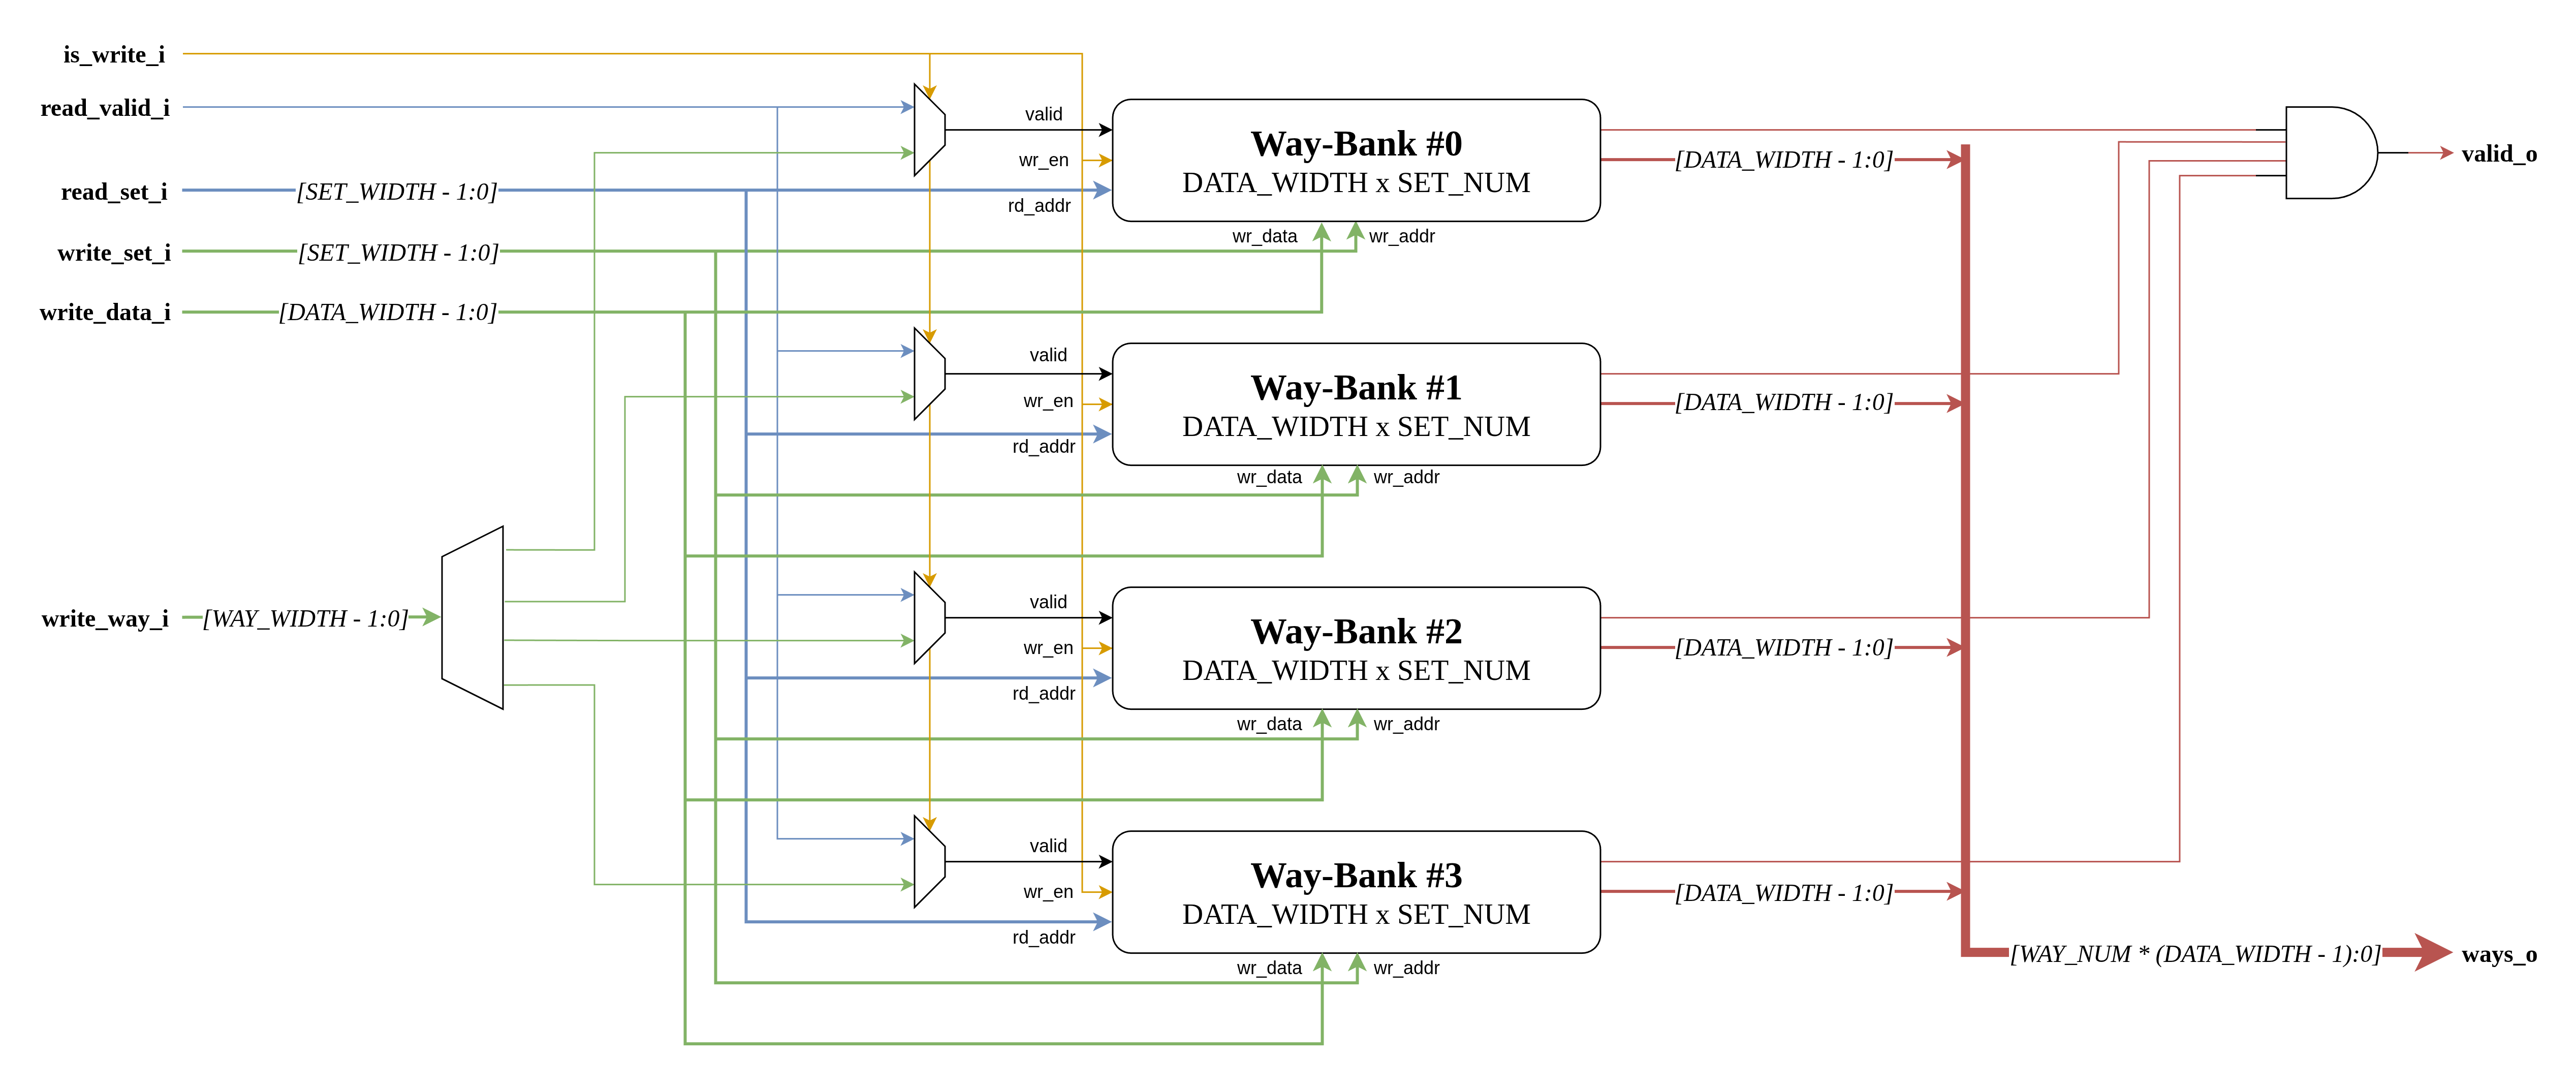
\includegraphics[width=16cm]{Data_Memory.png}
	\caption{Data Memory scheme (4-way cache)}
\end{figure}

\begin{table}[H]
	\centering
	\small
	\begin{tabularx}{\textwidth}{l c c X}
		\toprule
		\textbf{Parameter} & \textbf{Valid Range} & \textbf{Default} & \textbf{Description} \\
		\midrule
		
		\verb|DATA_WIDTH| &
		Positive integer &
		\verb|32| &
		Width of the data stored in each cache line. \\
		
		\verb|WAY_NUM| &
		Power of 2 &
		--- &
		Number of cache ways. \\
		
		\verb|SET_NUM| &
		Power of 2 &
		--- &
		Number of cache sets. \\
		
		\bottomrule
	\end{tabularx}
	\caption{Data Memory parameters}
	\label{tab:data_memory_parameters}
\end{table}

\begin{table}[htbp]
	\centering
	\label{tab:data_memory_ports}
	\small
	\begin{tabularx}{\textwidth}{l c c X}
		\toprule
		\textbf{Ports} & \textbf{Direction} & \textbf{Width} & \textbf{Description} \\
		\midrule
		\verb| read_valid_i | & Input & \verb| 1 | & Indicates a valid read request. \\
		\verb| read_set_i | & Input & \verb| SET_WIDTH | & Index of the cache set to be read. \\
		\verb| write_set_i | & Input & \verb| SET_WIDTH | & Index of the cache set to which the data is written. \\
		\verb| write_data_i | & Input & \verb| DATA_WIDTH | & Data to be written to the selected cache line. \\
		\verb| write_way_i | & Input & \verb| WAY_WIDTH | & Index of the way in which the input data is stored. \\
		\verb| valid_o | & Output & \verb| 1 | & Indicates that valid output data. \\
		\verb| ways_o | & Output & \verb| DATA_WIDTH * WAY_NUM | & Data stored in all ways of the requested cache set. \\
		\bottomrule
	\end{tabularx}
	\caption{Data Memory ports}
\end{table}
%%%%%%%%%%%%%%%%%%%%%%%%%%
%% T A G    M E M O R Y %%
%%%%%%%%%%%%%%%%%%%%%%%%%%

\subsection{Tag Memory}
\label{subsec:tag_memory}

The Tag Memory block encapsulates the multi-bank memory used to store cache tags and valid bits. Each bank stores the tag and valid bit corresponding to a specific way across all cache sets.

\begin{figure}[H]
	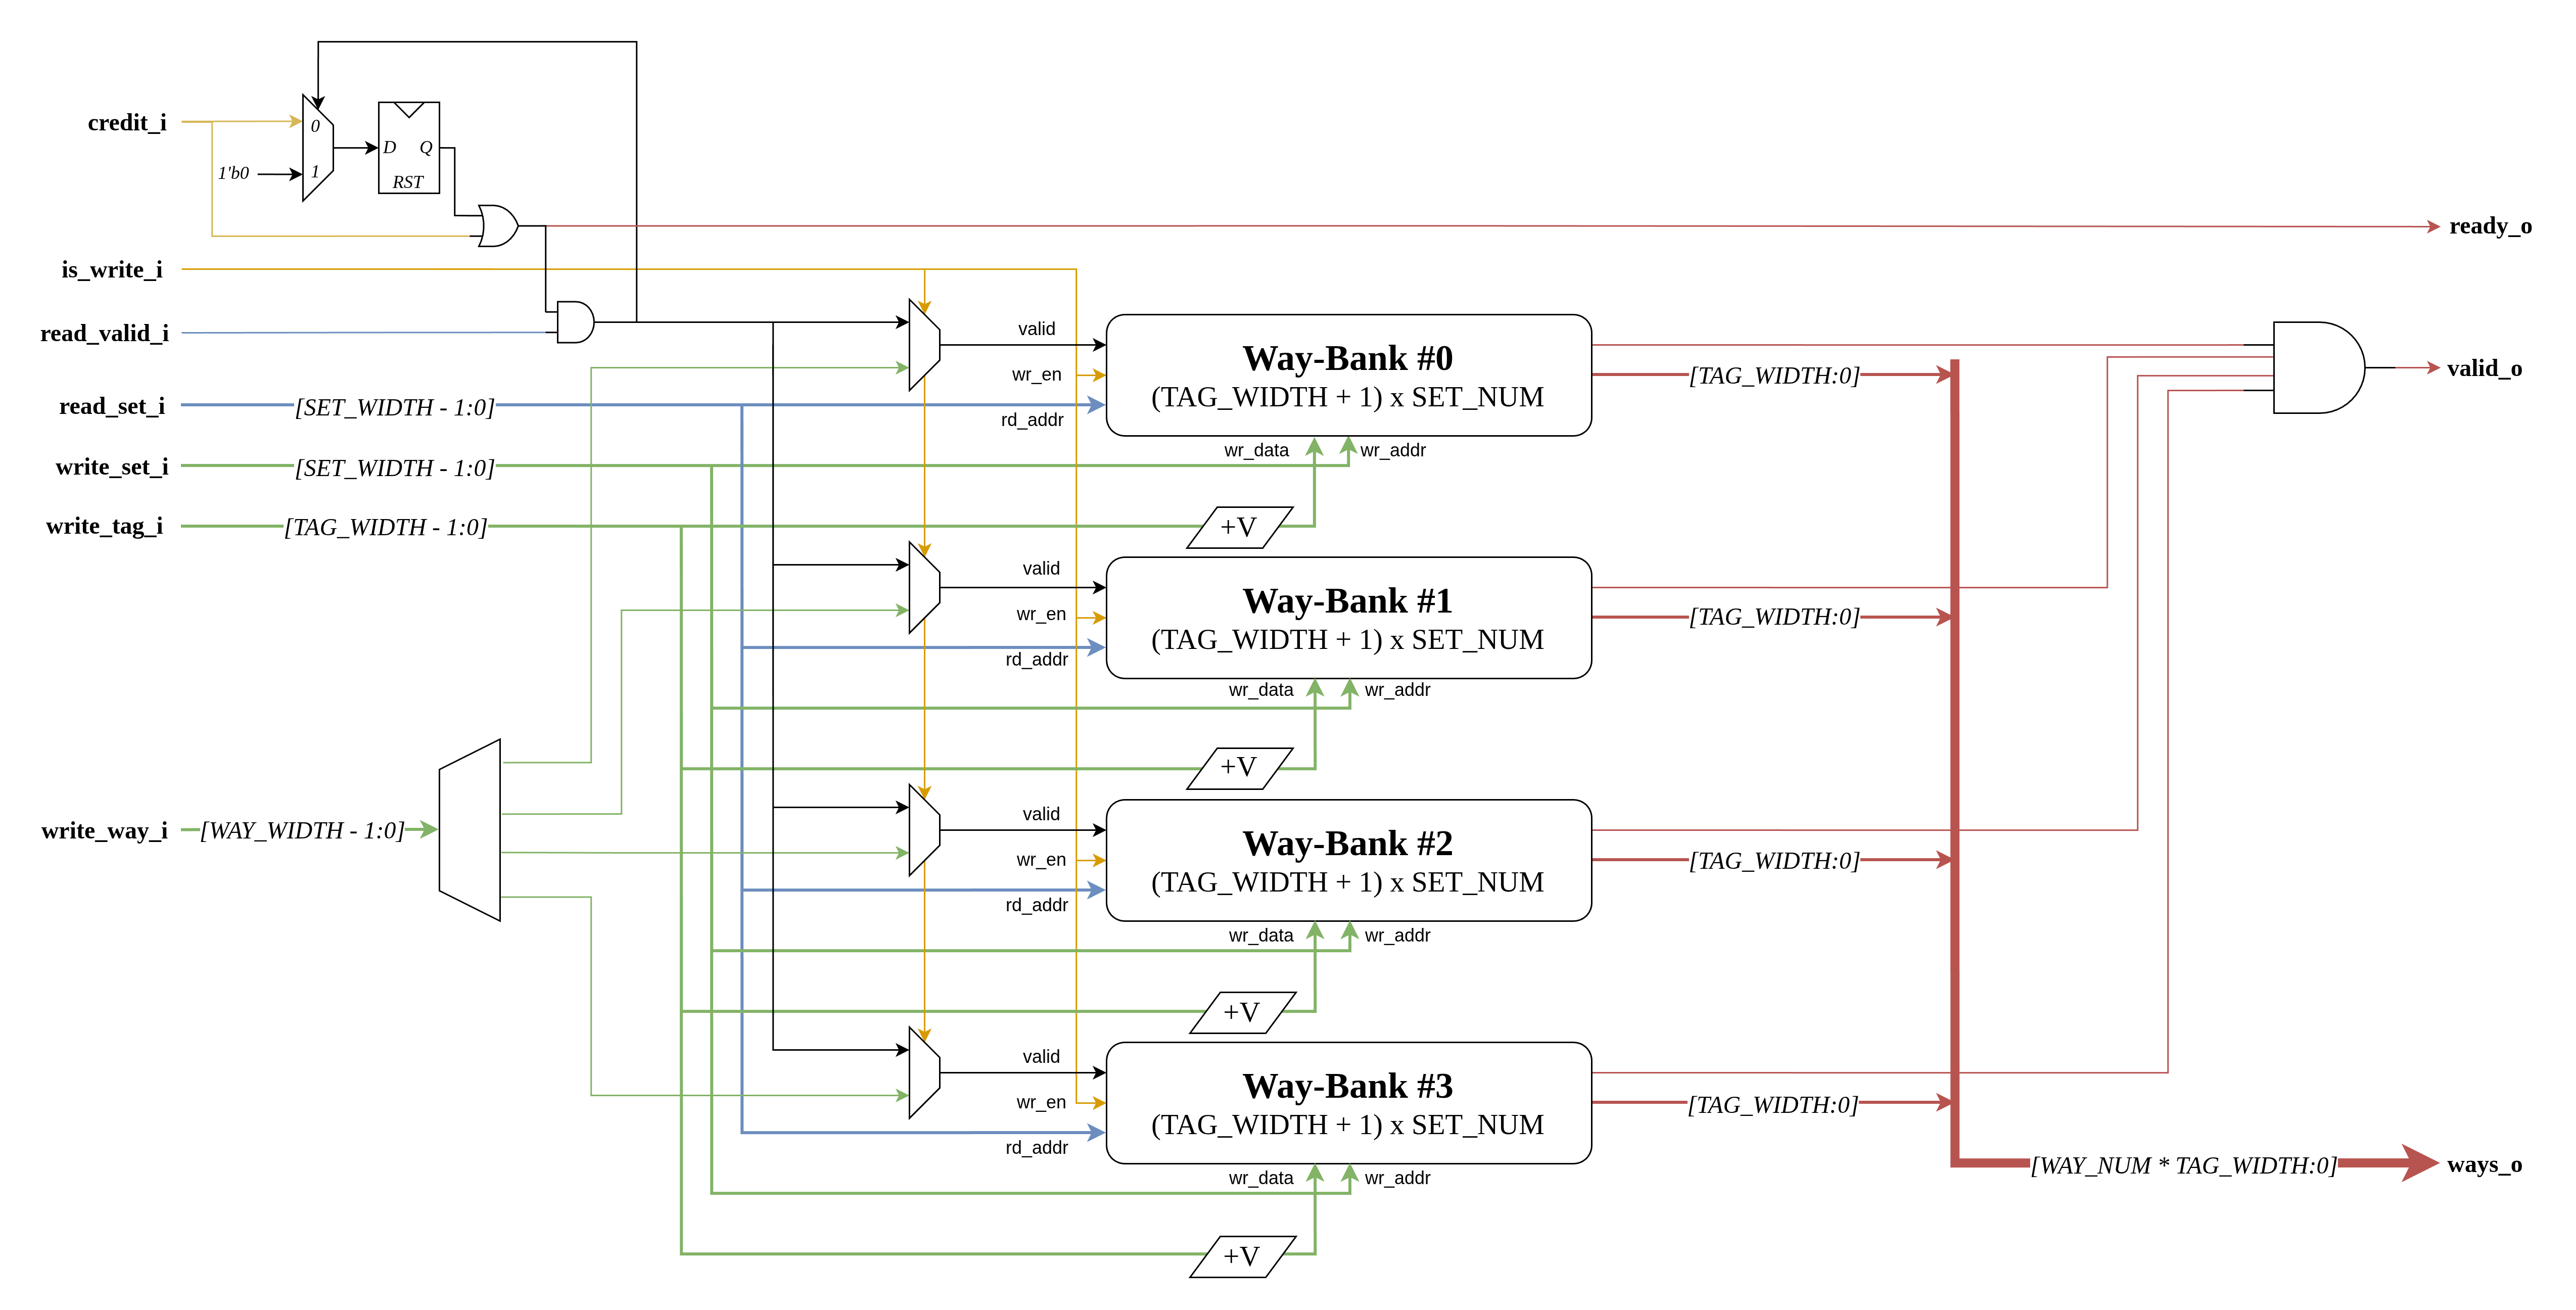
\includegraphics[width=16cm]{Tag_Memory.png}
	\caption{Tag Memory scheme (4-way cache)}
\end{figure}

Each memory bank is implemented as a pseudo-dual-port memory with a single memory access port that can be used for either a read or a write operation. Read requests are issued by the CPU-side cache logic, while write requests are generated by the cache control logic during cache operations. The access type is selected according to the current cache operation.

The Tag Memory also contains a credit counter that stores a single credit. A read request consumes the available credit, preventing a new read operation from being started until the current cache access has been completed. The credit is restored when the requested data is found in the cache or when a valid response is received from the external memory through the AXI4-Lite \verb|R| or \verb|B| channel. A restored credit can be used in the same clock cycle.

Write operations do not consume the credit and can therefore be performed independently of the credit counter.

Both read and write operations have a latency of one clock cycle.

\begin{table}[H]
	\centering
	\small
	\begin{tabularx}{\textwidth}{l c c X}
		\toprule
		\textbf{Parameter} & \textbf{Valid Range} & \textbf{Default} & \textbf{Description} \\
		\midrule
		
		\verb|TAG_WIDTH| &
		Positive integer &
		--- &
		Width of the tag stored in each cache line. \\
		
		\verb|WAY_NUM| &
		Power of 2 &
		--- &
		Number of cache ways. \\
		
		\verb|SET_NUM| &
		Power of 2 &
		--- &
		Number of cache sets. \\
		
		\bottomrule
	\end{tabularx}
	\caption{Tag Memory parameters}
	\label{tab:tag_memory_parameters}
\end{table}

\begin{table}[htbp]
	\centering
	\label{tab:tag_memory_ports}
	\small
	\begin{tabularx}{\textwidth}{l c c X}
		\toprule
		\textbf{Ports} & \textbf{Direction} & \textbf{Width} & \textbf{Description} \\
		\midrule
		\verb| read_valid_i | & Input & \verb| 1 | & Indicates a valid read request. \\
		\verb| read_set_i | & Input & \verb| SET_WIDTH | & Index of the cache set to be read. \\
		\verb| write_set_i | & Input & \verb| SET_WIDTH | & Index of the cache set to which the tag is written. \\
		\verb| write_tag_i | & Input & \verb| TAG_WIDTH | & Tag to be written to the selected cache line. \\
		\verb| write_way_i | & Input & \verb| WAY_WIDTH | & Index of the way in which the tag is stored. \\
		\verb| credit_i | & Input & \verb| 1 | & Indicates that a credit is available for a read request. \\
		\verb| ready_o | & Output & \verb| 1 | & Indicates readiness for a read request accept. \\
		\verb| valid_o | & Output & \verb| 1 | & Indicates that valid output data is available. \\
		\verb| ways_o | & Output & \verb| (TAG_WIDTH + 1) * WAY_NUM | & Tags and valid bits stored in requested cache set. \\
		\bottomrule
	\end{tabularx}
	\caption{Tag Memory ports}
\end{table}
%%%%%%%%%%%%%%%%%%%
%% A R B I T E R %%
%%%%%%%%%%%%%%%%%%%

\subsection{Arbiter}
\label{subsec:arbiter}

The Arbiter controls access to the memory interface shared by read and write requests. It implements a round-robin arbitration policy.

The arbiter maintains a priority state indicating which request type has priority when read (channel $a$) and write (channel $b$) requests are asserted simultaneously. When only one request is active, that request is granted regardless of the current priority. When both requests are active, the request with the current priority is granted. After a request is granted, the priority is updated to favor the other request type.

\begin{figure}[H]
	\centering
	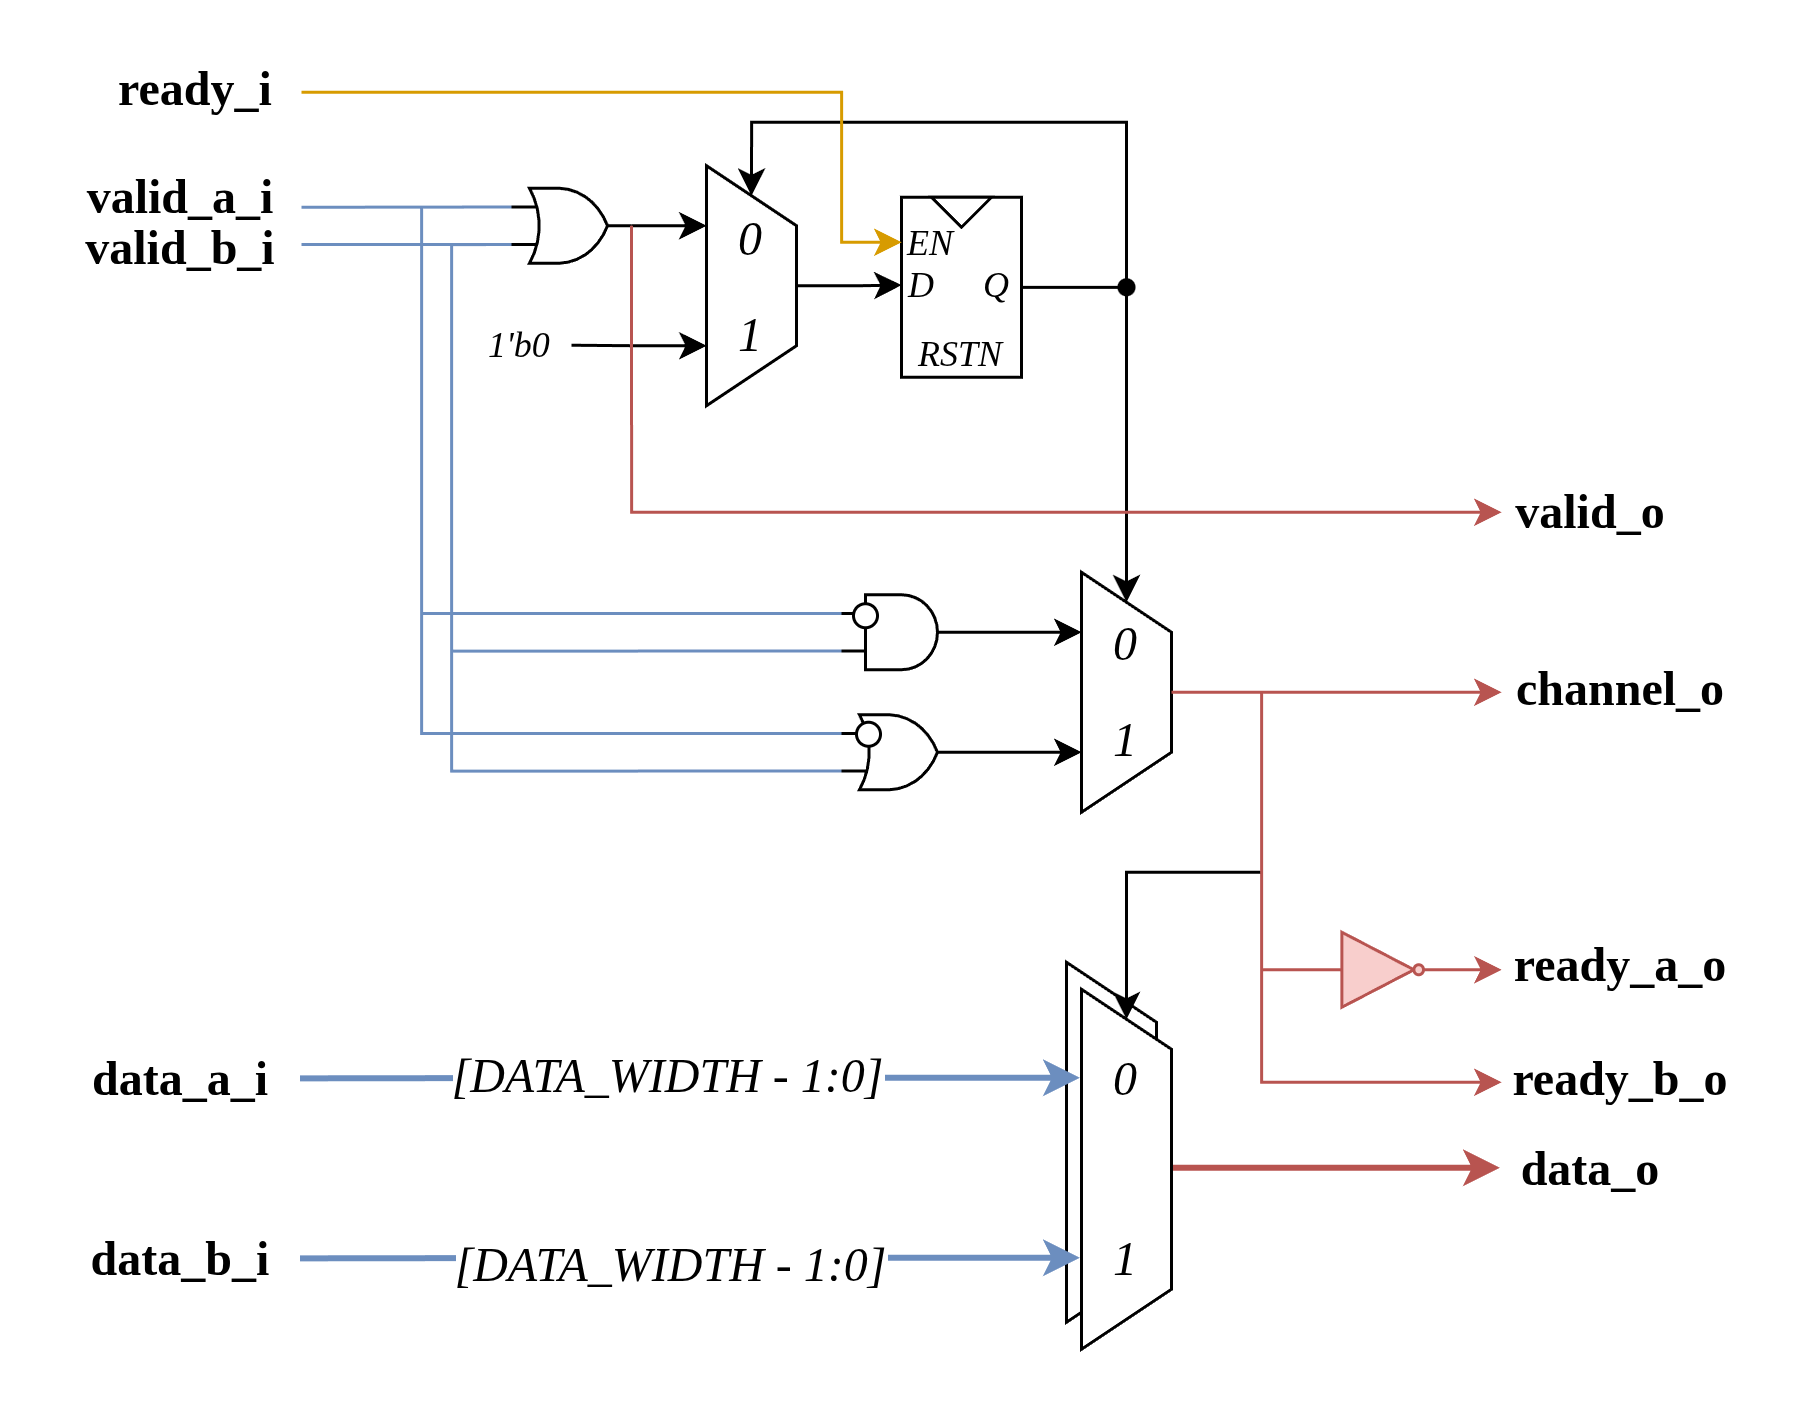
\includegraphics[width=7cm]{Arbiter.png}
	\caption{Round-Robin arbiter scheme}
\end{figure}

\begin{table}[H]
	\centering
	\small
	\begin{tabularx}{\textwidth}{l c c X}
		\toprule
		\textbf{Parameter} & \textbf{Valid Range} & \textbf{Default} & \textbf{Description} \\
		\midrule
		
		\verb|DATA_WIDTH| &
		Positive integer &
		\verb|32| &
		Width of the transaction data path. \\
		
		\bottomrule
	\end{tabularx}
	\caption{Round-Robin Arbiter parameters}
	\label{tab:round_robin_arbiter_parameters}
\end{table}

\begin{table}[H]
	\centering
	\label{tab:round_robin_arbiter_ports}
	\small
	\begin{tabularx}{\textwidth}{l c c X}
		\toprule
		\textbf{Ports} & \textbf{Direction} & \textbf{Width} & \textbf{Description} \\
		\midrule
		
		\verb|ready_i| &
		Input &
		\verb|1| &
		Indicates that the downstream logic is ready to accept the selected transaction. \\
		
		\verb|valid_a_i| &
		Input &
		\verb|1| &
		Indicates that a valid transaction is available on channel A. \\
		
		\verb|data_a_i| &
		Input &
		\verb|DATA_WIDTH| &
		Transaction data provided on channel A. \\
		
		\verb|valid_b_i| &
		Input &
		\verb|1| &
		Indicates that a valid transaction is available on channel B. \\
		
		\verb|data_b_i| &
		Input &
		\verb|DATA_WIDTH| &
		Transaction data provided on channel B. \\
		
		\verb|ready_o| &
		Output &
		\verb|1| &
		Indicates that arbiter is ready. \\
		
		\verb|valid_o| &
		Output &
		\verb|1| &
		Indicates that a valid transaction is available at the output. \\
		
		\verb|data_o| &
		Output &
		\verb|DATA_WIDTH| &
		Transaction data selected by the arbiter. \\
		
		\bottomrule
	\end{tabularx}
	\caption{Round-Robin Arbiter ports}
\end{table}
%%%%%%%%%%%%%%%%%
%% B U F F E R %%
%%%%%%%%%%%%%%%%%

\subsection{Buffer}
\label{subsec:buffer}

Buffer is a FIFO with a bypass path used to temporarily store incoming transactions. When the buffer is empty, a valid transaction can bypass the storage element and be passed directly to the output without additional latency. If the output is not ready to accept the transaction, it is stored in the FIFO and remains there until it can be forwarded.

\begin{table}[H]
	\centering
	\small
	\begin{tabularx}{\textwidth}{l c c X}
		\toprule
		\textbf{Parameter} & \textbf{Valid Range} & \textbf{Default} & \textbf{Description} \\
		\midrule
		
		\verb|DATA_WIDTH| &
		Positive integer &
		\verb|32| &
		Width of the transaction data stored in the buffer. \\
		
		\verb|FIFO_DEPTH| &
		Positive integer &
		\verb|1| &
		Maximum number of transactions that can be stored in the FIFO. \\
		
		\bottomrule
	\end{tabularx}
	\caption{Buffer parameters}
	\label{tab:buffer_parameters}
\end{table}

\begin{table}[H]
	\centering
	\small
	\begin{tabularx}{\textwidth}{l c c X}
		\toprule
		\textbf{Ports} & \textbf{Direction} & \textbf{Width} & \textbf{Description} \\
		\midrule
		
		\verb|valid_i| &
		Input &
		\verb|1| &
		Indicates that a valid transaction is available at the input. \\
		
		\verb|ready_o| &
		Output &
		\verb|1| &
		Indicates that the buffer can accept a new transaction. \\
		
		\verb|data_i| &
		Input &
		\verb|DATA_WIDTH| &
		Transaction data to be stored in the buffer. \\
		
		\verb|valid_o| &
		Output &
		\verb|1| &
		Indicates that a valid transaction is available at the output. \\
		
		\verb|ready_i| &
		Input &
		\verb|1| &
		Indicates that the downstream logic is ready to accept a transaction. \\
		
		\verb|data_o| &
		Output &
		\verb|DATA_WIDTH| &
		Transaction data provided at the output. \\
		
		\bottomrule
	\end{tabularx}
	\caption{Buffer ports}
	\label{tab:buffer_ports}
\end{table}
%%%%%%%%%%%%%%%%%%%%%%%%%%%%%%%%%%%%%%
%% S T A T I S T I C S    B L O C K %%
%%%%%%%%%%%%%%%%%%%%%%%%%%%%%%%%%%%%%%

\subsection{Statistics Block}
\label{subsec:statistics_block}

The Statistics Block provides cache hit and miss statistics for simulation and performance analysis. It receives hit and miss information from the \Comparator and maintains separate counters for cache hits and misses.

The block is enabled by the \verb|DEBUG_ON| parameter. When \verb|DEBUG_ON| is set to \verb|0|, the block is disabled and does not affect the cache implementation.

\begin{table}[H]
	\centering
	\small
	\begin{tabularx}{\textwidth}{l c c X}
		\toprule
		\textbf{Parameter} & \textbf{Valid Range} & \textbf{Default} & \textbf{Description} \\
		\midrule
		
		\verb|WIDTH| &
		Positive integer &
		\verb|32| &
		Width of the registers used to store the number of cache hits and misses. \\
		
		\bottomrule
	\end{tabularx}
	\caption{Statistics Block parameters}
	\label{tab:statistics_block_parameters}
\end{table}

\begin{table}[H]
	\centering
	\label{tab:statistics_block_ports}
	\small
	\begin{tabularx}{\textwidth}{l c c X}
		\toprule
		\textbf{Ports} & \textbf{Direction} & \textbf{Width} & \textbf{Description} \\
		\midrule
		
		\verb|valid_i| &
		Input &
		\verb|1| &
		Indicates that the current cache access is valid. \\
		
		\verb|hit_i| &
		Input &
		\verb|1| &
		Indicates whether the current cache access resulted in a hit. \\
		
		\verb|hit_count_o| &
		Output &
		\verb|WIDTH| &
		Number of recorded cache hits. \\
		
		\verb|miss_count_o| &
		Output &
		\verb|WIDTH| &
		Number of recorded cache misses. \\
		
		\bottomrule
	\end{tabularx}
	\caption{Statistics Block ports}
\end{table}
	%\newpage
	%\section{Waveforms}

This section illustrates the timing and sequence of AXI4-Lite transactions during different cache operations. The waveforms show the interaction between the CPU, the cache, and the external memory for cache hits, cache misses, and write operations.

\vspace*{\fill}
\begin{figure}[h]
	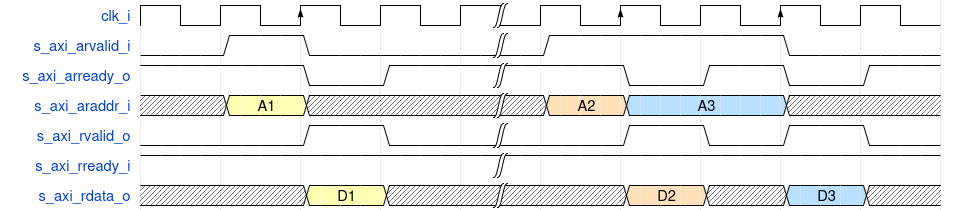
\includegraphics[width=16cm]{read_hit.png}
	\caption{Read hit waveform}
\end{figure}

\begin{figure}[h]
	\centering
	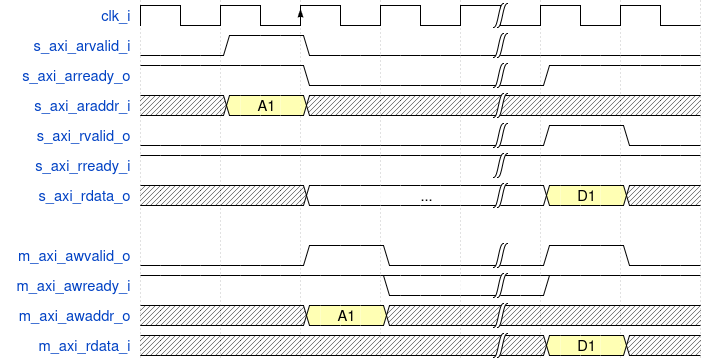
\includegraphics[width=12cm]{read_miss.png}
	\caption{Read miss waveform (without eviction)}
\end{figure}
\vspace*{\fill}

\newpage

\vspace*{\fill}
\begin{figure}[h]
	\centering
	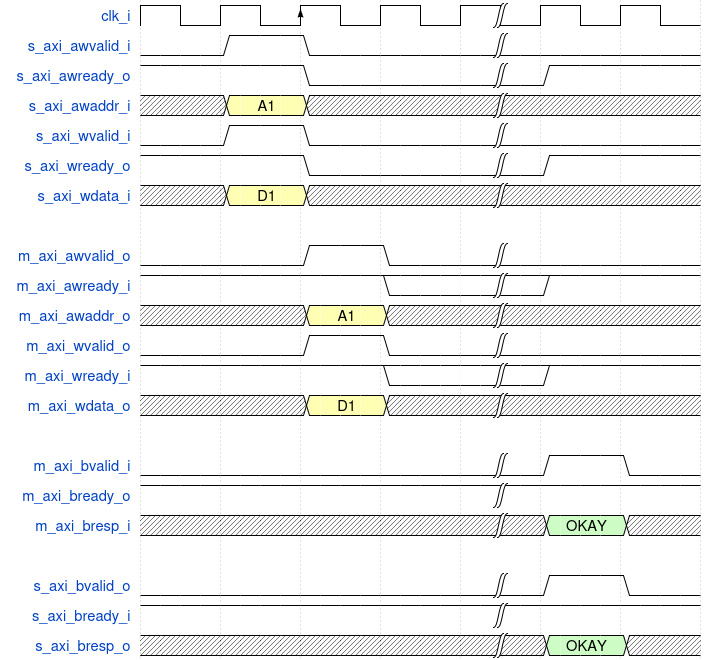
\includegraphics[width=13cm]{write_hit.png}
	\caption{Write waveform}
\end{figure}
\vspace*{\fill}

\newpage

\vspace*{\fill}
\begin{figure}[ht]
	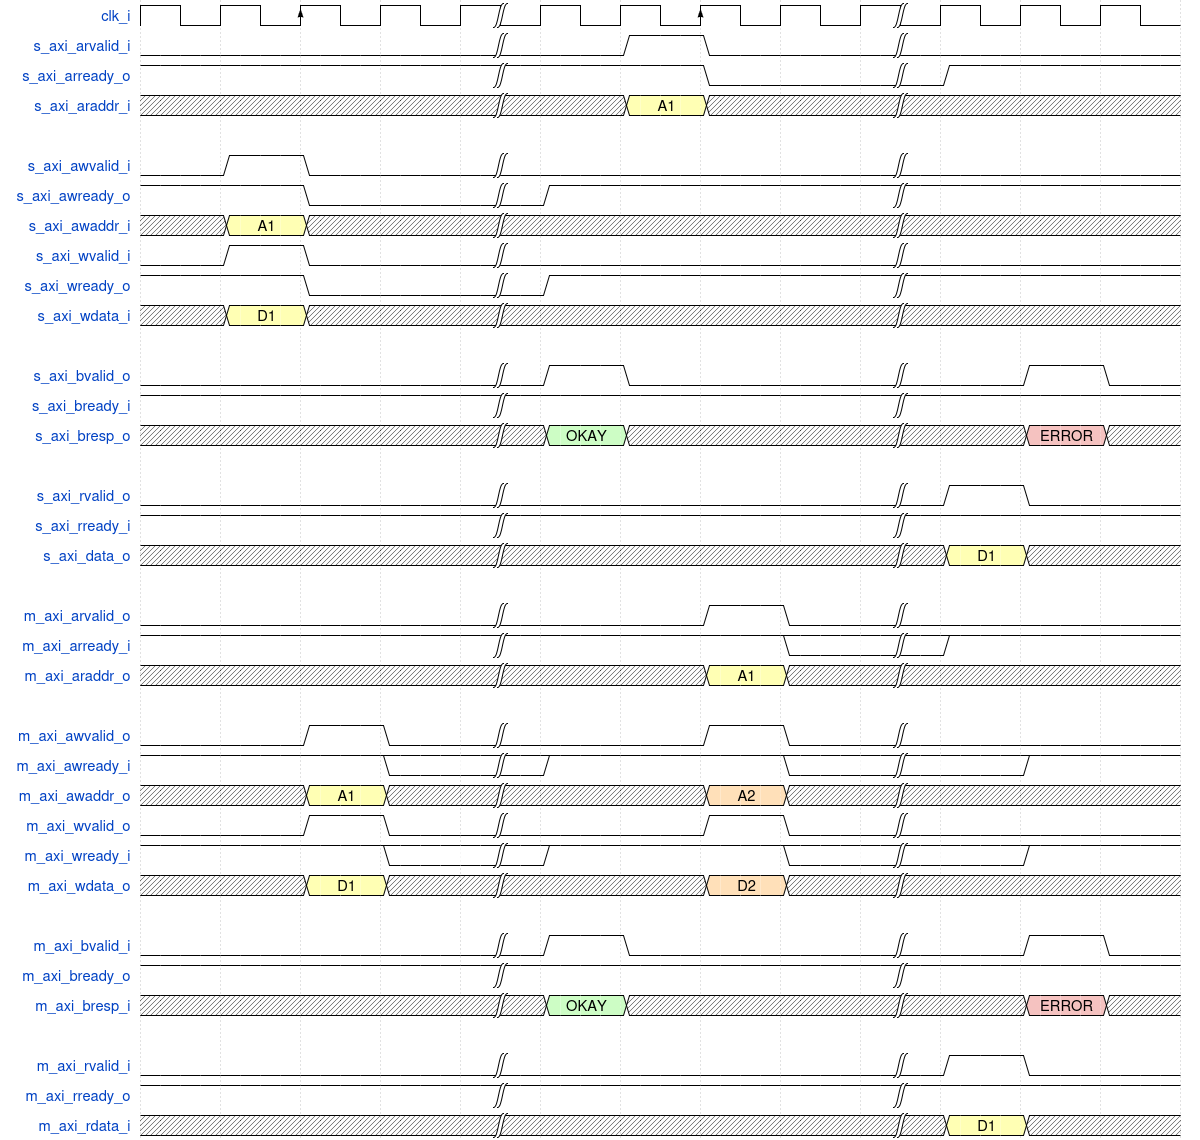
\includegraphics[width=17cm]{comb.png}
	\caption{Sequence of a write and read operation to the same address (the address was initially present in the tag memory)}
\end{figure}
\vspace*{\fill}
	
\end{document}
